\documentclass[fleqn,10pt]{wlscirep}
\usepackage[utf8]{inputenc}
\usepackage[T1]{fontenc}
\usepackage{placeins}
\usepackage{graphicx}
\usepackage{lscape}
\usepackage{todonotes}
%\usepackage{xcolor}
\usepackage{multirow}
\usepackage[table,xcdraw]{xcolor}
\usepackage{lscape}
\usepackage{adjustbox}

\newcommand{\beginsupplement}{%
        \setcounter{table}{0}
        \renewcommand{\thetable}{S\arabic{table}}%
        \setcounter{figure}{0}
        \renewcommand{\thefigure}{S\arabic{figure}}%
     }
\newcommand{\gp}[]{\textsc{gp }}

%\title{Prioritization for diagnosis through whole-genome sequencing of product of conception from idiopathic pregnancy losses }
\title{Paper Title}

\author[1+]{Silvia Buonaiuto}
\author[2+]{Imma Di Biase}
\author[3+]{Valentina Aleotti}
\author[4]{Adriano De Marino}
\author[1]{Gianluca Damaggio}
\author[5]{Marco Chierici}
\author[6]{Madhuri Pulijala}
\author[2]{Palmira D’Ambrosio} 
\author[2]{Gabriella Esposito}
\author[6]{Qasim Ayub}
\author[5]{Cesare Furlanello}
\author[7]{Nicole Soranzo}
\author[3]{Michele Rubini}
\author[4]{Antonio Capalbo}
\author[2]{Sebastiano Di Biase}
\author[1*]{Vincenza Colonna}
%\author[]{{\color{blue} nomi memorial exomes} }
\affil[1]{Affiliation, department, city, postcode, country}
\affil[2]{Affiliation, department, city, postcode, country}
\affil[*]{Correspondence: vincenza.colonna@igb.cnr.it (V.C.)}
\affil[+]{these authors contributed equally to this work}

%\keywords{Keyword1, Keyword2, Keyword3}

%\begin{abstract}

%PL impact on health - current diagnosis - It is estimated that up to 50\% of cases of PL do not have a clearly defined etiology.\cite{practice2012evaluation} - importance of diagnosis made on PoC: screening pre-IVF, genetic counselling for parents, research \\

%Current methods of diagnosis - What is missed: target on small-size genetic variants that causes PL  - How is this possible: diagnosis by whole genome sequencing,  not a routine, the protocol needs to be developed through large-scale projects  \\

%We present a collection of PL that complies to standards that we want to use for a pilot project - We use this collection to 1. draft a pipeline for samples prioritization before performing whole-genome sequencing 2. Estimate the size of the samples to be collected for large-scale studies\\

%We find: 20\% of samples goes to sequencing useful for determining sequencing costs and capabilities 

%\end{abstract}
\begin{document}

\flushbottom
\maketitle
% * <john.hammersley@gmail.com> 2015-02-09T12:07:31.197Z:
%
%  Click the title above to edit the author information and abstract
%
\section*{Introduction}
\gp 
%Human reproduction is highly ineffective and it is estimated that 10-20\% of all pregnancies end in early miscarriage or early pregnancy loss (PL) during the first trimester [REF SILVIA] and up to 50\% of cases of RPL do not have a clearly defined etiology\cite{practice2012evaluation}. Miscarriage is defined as the death of the fetus within 20-28 week of gestation\cite{pmid27994187, pmid25055407, pmid25944391, pmid11821293, stephenson2002cytogenetic, pmid25681385, pmid29858908}. Recurrent pregnancy loss (RPL) is defined as the loss of two or more consecutive pregnancies\cite{green2019review}. RPL has a high impact on public health since it affects up to 3-5\% of couples[REF PER QUESTO]. For 50-60\% of RPL cases the cause are known to be structural genetic, endocrine, anatomic, thrombophilic, autoimmune, and environmental factors, however for the remaining 40-50\% the causes are unknown\cite{pmid27994187, pmid25944391, pmid11821293, stephenson2002cytogenetic, pmid22796359, pmid22672580, pmid25681385, gaboon2013recurrent, pmid30642578}.\\


%The diagnosis of miscarriages is based on embryo heart activity and gestational sac features revealed by ultrasonography\cite{doubilet2013diagnostic}. Nevertheless, diagnosis take place only after the death of the embryo, and only few cases there are followed-up to understand the genetic causes with techniques that can discriminate anouplidies (kariotyping, quantitative PCR) or large deleterious copy number variants (comparative genomic hybridization), while no information is available on small-size DNA changes incompatible with life. Therefore, the current ability of inform prognosis and manage decision in cases of perinatal lethality is limited, with important consequences in counseling for RPLs and \textit{in-vitro} fertilization.\\

%Among PL caused by genetic defects, it is estimated that 50-70\% [check PERCENT] is due to meiotic chromosome segregation errors, whose frquency increases with increasing maternal age\cite{pmid30393965, pmid10864550, pmid20041396}. Sperm DNA fragmentation caused by oxidative stress also causes PL through impairment of placentation \cite{pmid2972074, pmid30448091, pmid30602480}. %as well as increased mutation rate in sperm that increases with male age\cite{kong2012rate}. 
%To date, PLs are studied using parental genetic information \cite{laisk2019genetic, pereza2017systematic}. Only a few studies have focused on deep understanding of the genetic causes through the analysis of the fetal genome sequence\cite{filges2015exome}[ADD REF]. However, these few cases never considered whole genome sequencing but rather concentrated on restricted target regions related to specific medical cases. Therefore, very little is known about the genetic mutations that effectively cause the death of the embryo and there is the need for large scale projects that systematically target small-size genetic mutations. % to help understanding unexplained PLs. 


%In this study we develop a pipeline for selecting cases of idiopathic PL to be studied through whole-genome sequencing of DNA from product of conception (PoC).  \\
%We find that... \\
%Our study will facilitate the development of a larger-scale project for developing molecular diagnosis of PL. 


%The aims of this study is to identify genetic variants to cause miscarriages and improve prenatal diagnosis. We analyze DNA obtained from tissue of chorionic villi from cases of SA and RM, comparing with controls, voluntary termination of pregnancy (VTP)[\cite{pmid28352815}]. In the first phase, the data on habits and health status of women subjected to abortion were analyzed, with particular attention to gestational age, BMI, menarche age, age of women at time of the pregnancy, use of alcohol, drugs or coffeine etc. An initial stratification of the samples was performed based on the results of these data. Subsequently the samples were analyzed by qfPCR, in order to remove from the miscarriage study, the samples with chromosomal anomalies. In the second phase a CGH array was performed to exclude anomalies not visible to the qfPCR. In the third phase, the fetal DNA sequences that were found to be suitable, have been analyzed.



 

%The protocols provide a dedicated and focused service to couples who already had experience of  RPL, so it doesn’t prevent from a new event of miscarriage. The goal of the pregnancy loss is have a prevention center, as write in study of Bruce K.Young, 2019. An essential part of the management of couples with recurrent miscarriage is to give trustworthy advice on the prognosis for the next pregnancy for the couples to be able to decide for or against further pregnancy attempts. In the field of recurrent miscarriage, however, a distinct problem is the lack of comparability between estimates of the chance of subsequent successful pregnancy outcomes reported in various studies. The chance of live birth in the next pregnancy in women with three, four, and five previous miscarriages has been reported variably to be between 63 and 87\%, 44 and 73\%, and 25 and 52\%, respectively. Nowadays, the first visit after referral for RPL should allow time for the clinician to review the patient’s history, which includes medical, obstetric, and family history, but also information on lifestyle of both the male and female partner. Studies have suggested an impact of the following lifestyle factors on the risk of RPL: smoking, excessive alcohol consumption, excessive exercise and being overweight or underweight. In addition to lifestyle factors, information should be collected on a previous diagnosis of medical conditions that may be associated with RPL, including thrombophilia, PCOS, and diabetes, or a family history of hereditary thrombophilia. Medical and family history could be helpful in deciding which investigations are relevant for the individual patient (age, fertility/sub-fertility, pregnancy history, family history, previous investigations and/or treatments). However, no studies have been performed that could advise clinicians on which diagnostic tests are relevant for a specific patient and, more importantly, which are not [\cite{pmid29858908, pmid22183209, pmid22835448, pmid29720743}].



%Genetic abnormalities of the conceptus are a recognized cause of SA and RPL. In literature the prevalence of chromosome abnormalities in this cases was 40-50\%. Determining the chromosomal status of pregnancy tissue from women with recurrent pregnancy loss may provide them with a cause or reason for the particular loss being investigated. No clear effect of genetic testing of the pregnancy tissue on prognosis (subsequent live birth) has been described so far and the role of genetic analysis of pregnancy tissue should be further elaborated within a prognostic model. If women are offered genetic analysis of pregnancy tissue, they should be aware of the issues as mentioned.


%It was decided to recommend parental karyotyping in RPL couples only after an individual risk assessment. Parental karyotyping can be recommended based on genetic history (for instance in case of the previous birth of a child with congenital abnormalities, offspring with unbalanced chromosome abnormalities in the family, or detection of a translocation in the pregnancy tissue). For other couples, the benefit of the test is limited as the chances of finding an abnormality are very low: in couples with female age above 39, less than three pregnancy losses and a negative family history, the chance of being a carrier of a translocation is very low.
%Parental karyotyping may provide couples with a possible contributing factor and prognostic information for the subsequent pregnancy. Regarding prognosis, couples should be informed that, even if a parental abnormality is found after karyotyping, the cumulative live birth rates are good, as are the chances of a healthy child, despite a higher risk of a subsequent pregnancy loss. Furthermore, they should be informed of the limitations of karyotyping, including that karyotyping does not predict unbalanced translocation in next pregnancy.

\section*{Results}
To understand genetic susceptibility to miscarriage we studied the genome of forty-six miscarried embryos. The embryos gestational age at pregnancy termination, calculated as the interval between the pregnancy termination date and the last menstruation date, ranges from 7.14 to 19.43 weeks (median is 10.3 weeks). Twenty-one embryos classifies as the product of recurrent miscarriages \cite{eshre2018eshre}. The mothers of the embryos are mostly of European origin (87\%) and their median age at the date of collection was 36.7$\pm$5.9 years, with no significant difference between first and recurrent cases (Figure \ref{fig:embryostats}, Mann–Whitney p-value=0.02). For the mothers of the embryos medical records report no major comorbidities. Folic acid was taken by 71\% of the mothers with no difference between first and recurrent cases (Figure \ref{fig:embryostats}, Chi-square p-value=0.96). Median body mass index and menarche age are comparable between first and recurrent cases, as well as comparable to a group of control women (Figure \ref{fig:embryostats}). Altogether, from the available medical records, we suppose that the recruited mothers of the embryos were in the range of healthy adult individuals. %The nine women with recurrent clinical miscarriage had an average of 4 previous clinical miscarriages (SD=2.7, range 3-11), average age of 33 years (SD=6; range 23-40), average BMI within the range of normality (24.6; SD=3.9), and ovarian reserve in the XX percentile by the mean age (Anti-Mullerian hormone mean 2.1 pmol/l; SD=2.1).

It is known from literature that roughly xx\% of the miscarriages in the first trimester are due to large chromosomal aneuploidies, such as trisomies or deletions of large chromosomal chunks \cite{goddijn2000genetic,zhang2009genetic}. In this study we want to focus on cases in which the genome is euploid, therefore the forty-six embryos were screened for chromosomal aneuploidies prior to whole-genome sequencing. We find that 32.6\% of samples were euploid and could be sequenced while 56.6\% of the embryos presented aneuploidies (Figure \ref{fig:presequencing}).The most common aneuploidy in our data set is the trisomy of chromosome 22 (26.9\%), followed by trisomy of chromosome 16 (15.4\%). In particular, a first round of detection of aneuploidies on chromosomes 13, 15, 16, 18, 21, 22, X, and Y through Short Tandem Repeats analysis discarded 45.7\% of samples, %These types of repeats (tetra- or penta-nucleotide) are often expected to be found in heterozygosis, therefore triploidy is assumed when three alleles are found at several markers along a chromosome (complete) or part of it (partial). Similarly, uniparental disomy for a targeted region or chromosome is assumed when only one parental allele is amplified. 
and a subsequent analysis through comparative genomic hybridization and copy number variation detection form low-coverage sequencing discarded another 10.9\% of the samples. Finally, a number of embryos (10.9\%) dropped off the analysis due to low-quality DNA or maternal contamination. 

After ascertaining euploidy, %the exome of the nine women was sequenced using Agilent SureSelect whole-exome capture and Illumina sequencing technology on the NovaSeq 6000 Series Sequencer(Next Generation Solutions, Hong Kong, China), while 
the whole genome of ten embryos was sequenced using Illumina short-reads at 30X coverage. In the set of embryos genomes, we identified 11M single-nucleotide polymorphisms (SNPs) and 2M small insertions or deletions (indels).%, while from the exome data of the women we identified 1.7M SNPs and 276k indels.
%In the set of embryos genomes, we identified 11041,557 single-nucleotide polymorphisms (SNPs), 1980256 small insertions or deletions (indels), and XX copy number variants (CNVs). In the set of women we identified 1738895 SNPs and 275652 indels.


%5493 genes in hgdp for exomes
%1323 discarded and 76% retained
\subsection*{Prioritization of genetic variants in coding genomic regions} 
We developed the \gp pipeline to prioritize putatively damaging genetic variants from sequencing data. \gp takes as input genomic variants information from cases and controls (including the per-individual allelic counts) in form of a vcf file and outputs a table of variants prioritized according to user-defined parameters. \gp uses functional annotations of genomic variants, information from publicly available sequence data of presumably healthy individuals, and, if available, knowledge of genes involved in the trait under study. \gp currently analyze coding regions and performs four filtering steps (Figure \ref{fig:pipeline}). The first filter (Filter I) retains variants based on: (i) a user-defined threshold of allele frequency in control populations; (ii) an overall impact on the gene product classified as moderate or high [REF]; (iii) the combined property of being putatively damaging (quantified by the CADD score\cite{rentzsch2019cadd}) and located in genes intolerant to loss of function (determined by the pLI score [REF]). In addition it is possible to incorporate one or more user-defined lists of genes relevant to the trait under study, and take this into account when applying Filter I. Variants retained by Filter I (hits) are further filtered to control for false positives with Filters II and III. Finally, Filter IV excludes private variants with read depth outside the range found in non-private ones.   

%Filter II removes variants in genes with too many hits. Filter III controls for the chance of random occurrence of genes based on replicates of Filter I analysis in a large control population. In practice it removes all the genes that pass Filter I a user-defined-fraction of times across a user-defined-number of replicates. 

We applied the \gp pipeline to data from the high-coverage whole-genome sequences of genomic DNA of the embryos. For Filter I we set allele frequency <0.05\% in the 1000 Genomes [REF] and gnomAD[REF] reference populations, while the functional effect of the variant within the gene context was taken into account in two ways: either selecting for putatively deleterious variants (CADD score >90th percentile) in genes highly intolerant to loss of function (pLI score >0.9), or selecting for variants in genes known to be involved in early embryonic development. In particular for this last option we included five lists of genes, namely genes involved in embryo development (Gene Ontology GO:0009790), genes lethal during embryonic stages \cite{dawes2019gene}, essential for embryo development \cite{dawes2019gene}, genes discovered through the Deciphering Developmental Disorders project [REF DD], and a manually curated list of candidate genes known to be involved in miscarriages. We requested the variant to satisfy one or both these criteria: (i) be in a gene present in at least two of the five lists or (ii) have CADD score above the 90th percentile and be in a gene with pLI>0.9. Overall, filter I retained 1,038 and 728 variants (hits) in embryo and mothers, respectively.   

Filter II removed variants in genes with >5 hits. With few exceptions, we observed that the majority of genes (99th percentile) has less than five hits, even if there is no significant correlation between number of hits and gene length (Spearman r=XX p-value=xx, Figure \ref{fig:filters}A). Genes with >5 hits have more paralogues than genes with <5\% (???) and hits in gene with >5 hits are enriched for private variants  We concluded that variants found in gene with more than five hits are likely to be sequencing and alignment artifacts and therefore are discarded. 

For Filter III we used as control population 929 individuals from the Human Genome Diversity Project (HGDP, [REF]) from which we resampled 100 times ten individuals. On each resampled set we performed Filter I analysis and recorded the genes that were retained. Overall 5,488 unique genes were retained in controls with different frequencies in samples across replicates (Figure \ref{fig:filters}B ). When considering the 95th percentile, 1,531 genes are found >5\% of times across replicates, therefore hits within these genes were removed by filter III. %Because the criteria used for Filter I were identical between embryos and mothers, and because the numerosity was very similar, we performed resampling only once and applied the outcome to both analyses.

Filter II and III, retained 447 hits of which 21\% are private with respect to 1000 Genomes and gnomAD data sets. Despite comparable read depth between private and non-privates variants (Figure \ref{fig:filters}C-D, KS test p-value=XX, F test p-value=XXX), to further control for possible artifacts due to scanty coverage, we applied a further filter that removes hits which are private variants with read depth outside the range found in non-private ones.   



%The genes prioritized in women are slightly enriched for genes belonging to mitochondrial translation initiation (R-HSA-5368286), elongation (R-HSA-5389840), and termination (R-HSA-5419276) pathways (p-value=0.0002, Benjamini-Hochberg adjusted p-value=0.0574, FDR=0.056). This enrichment is due to eight genes selected by \gp in six women due to missense mutations (Table \ref{tab:mito}).  --More about the eight genes %(\textit{MRPL15}, \textit{MRPL34}, \textit{MRPL37}, \textit{MRPS15}, \textit{MRPS21}, \textit{MRPS23}, \textit{MRPS28}, and \textit{OXA1L}) 

%%%%%%%%%%%%%%%%%%%%%%%%%%%%%%%%%%%%%%%%%%%%%%%%%%%%%
\subsection*{Properties and biological significance of the prioritized variants and genes} 

After all filters, \gp prioritize 439 unique variants in 399 genes that code for 980 transcripts. Almost all the prioritized genes (n=378) have an OMIM accession number and 18.8\% of them were not in the lists of candidate genes used by \gp as input during the prioritization, demonstrating that \gp is robust to detection of genes never investigated before in relationship to the phenotype under study. 

Nine genes are involved in the pathway of mitochondrial translation (Reactome identifier R-HSA-5368287) and this number represent a significant 4.9 fold enrichment over random expectations (Table \ref{tab:rectomepathways} over-representation test p-value=1.45E-04, FDR=3.00E-02). Similarly, we observe over representation of genes involved in cell cycle checkpoints (R-HSA-69620) and signaling by Rho GTPases (R-HSA-194315). With reference to the cellular compartments where the gene product are expressed, we observe a 7.7 fold significant enrichment (p-value 7.82E-04, FDR=4.24E-02) of protein expressed in the mitotic spindle pole or in associated complexes (Table \ref{tab:GOcellcomponentcomplete}), among which the product of \textit{STAG2} for which we observe an high-impact mutation in one embryo from this study.  

Finally, seven genes (\textit{BHLHE40},\textit{DBN1}, \textit{FOXA1}, \textit{HSPD1}, \textit{PLXNA3}, \textit{SLC35A2}, \textit{SRF}) were previously identified as essential genes in copy-number variable regions from the analysis of hundreds of miscarried fetuses \cite{chen2017characterization} % Among them, \textit{HSPD1} for which two embryos from this study share an heterozygous missense mutation
% BHLHE40
% DBN1
% FOXA1
% HSPD1 in two samples 
% PLXNA3
% SLC35A2
% SRF

In the embryos 4.1\% of the prioritized variants are stop gains/loss, frameshift indels, and variants that disrupt splicing sites, all classified as having high impact on the gene products, while missense mutations prevail among the variant with moderate effect (Figure \ref{fig:resembryo}A). Averages per embryos are 48.9$\pm$8.0 genomic variants in 47.8$\pm$7.7 genes coding for 113.5$\pm$24.6 transcripts (Figure \ref{fig:resembryo}B). For almost all genes \gp retains one variant per embryo, with few exception (five cases with two e and one with three variants per gene), as shown in Figure \ref{fig:resembryo}B, where the allele dosage and impact are also shown. %--Shared genes/variants 

\subsubsection*{Mutations in \textit{STAG2},\textit{TLE4}, \textit{FMNL2}, and \textit{FRMPD3} in the embryos} 
%validation merigen? 
The male embryo AS030 carries one extremely rare T>G transversion (rs913664484, G frequency is 4.7e-05 in 42.7k individuals from gnomeAD [REF]) that changes one of the two basis at the 5' end of the first intron of the \textit{STAG2} gene (ENSG00000101972), altering a splice site (splice donor variant, high impact). \textit{STAG2} is on the X chromosome and codes for the cohesin subunit SA-2 \cite{cuadrado2020specialized}. Cohesins are ring-shaped protein complexes that brings into close proximity two different DNA molecules or two distant parts of the same DNA molecule \cite{mcnicoll2013cohesin}. In mouse, inactivation \textit{Stag2} causes early embryo lethality \cite{de2020essential}, and  mutations in \textit{STAG2} have been discovered in children with developmental disorders (REF DDD). Interestingly, only mildly-deleterious mutations have been found in males \cite{mullegama2019mutations}. 

The embryo AS036 carries an heterozygous missense G>C mutation (rs41307447) in the \textit{TLE4} (ENSG00000106829, synonym \textit{GRG-4}) gene that causes a substitution of a polar amino acid with another polar amino acid (Ser>Tre) in the 7 exon of the gene, corresponding to a low complexity domain of the protein. The rs41307447 polymorphism is tolerated (SIFT score 0.18) and supposed to be benign (PolyPhen score 0.003), nevertheless the \textit{TLE4} gene is classified as highly intolerant to loss of function (pLI score 0.999) and the CADD score associated to rs41307447 is in the 99.8th percentile. 
\textit{TLE4} is a trascriptional repressor of the Groucho-family expressed in the embryonic stem cells where it repress naive pluripotency gene \cite{laing2015gro} and it is a direct transcriptional target of Notch \cite{menchero2019transitions}. \textit{TLE4} is also expressed in the extravillous trophoblasts \cite{meinhardt2014wnt} where it is part of the Wnt signaling pathway that promotes implantation, trophoblast invasion, and endo-metrialfunction \cite{sonderegger2010wnt}. Notably, a recent association study in a cohort of 750 cases of women experiencing recurrent miscarriages found a signal on chromosome 9 (rs7859844) in a genomic region physically interacting with \textit{TLE4} \cite{laisk2019genetic}, corroborating the hypothesis of association between variation in \textit{TLE4} and miscarriages. 

% AS093, AS090, AS087, AS065, AS036) 
Five embryos share one copy of an haplotype composed of two T alleles 4bp apart (rs866373641, rs750755379) in the \textit{FMNL2} gene (Table \ref{tab:fmnl2}). The two alleles exists at moderate-to high frequency in human populations (Table \ref{tab:fmnl2}) and are in perfect linkage disequilibrium (r\textsuperscript{2}=1) in the embryos, as well as in other cohorts (r\textsuperscript{2}= hgdp etc..). Women in this study .... 
We validated the association between the TT haplotype and phenotypic traits related to miscarriages in --UKBB 
In addition to the two mutations described above, the embryo AS065 has a missense mutation in phase (rs189416564, c.758C>G, p.Leu110Val, deleterious SIFT=0, probably damaging, PolyPhen = 0.969) 
\textit{FMNL2} codes for a formin-related protein and has 4 transcripts (splice variants). It is located on chromosome 2:152,335,174-152,649,826 forward strand. Formin-related proteins have been implicated in morphogenesis, cytokinesis, and cell polarity. \textit{FMNL2}, in particular, is expressed in the fetus in the cytoplasm of brain, spinal cord, and rectum\cite{lizio2015gateways}. \textit{FMNL2} is an elongation factor of actin filaments that drives cell migration by increasing the efficiency of lamellipodia protrusion \cite{block2012fmnl2} --more on FMNL2
    %It is implicated in cytoskeleton organization (GO:0007010), regulation of cell shape (GO:0008360), cellular component organization (GO:0016043), cell migration (GO:0016477), regulation of cell morphogenesis (GO:0022604), actin cytoskeleton organization (GO:0030036), cortical actin cytoskeleton organization (GO:0030866).

Two embryos (male AS065, female AS006) share a stop gain mutation in the X linked gene \textit{FRMPD3}, highly intolerant to loss of function (pLI = 0.91). Expressed in brain, ovary. thyroid (PROTEIN ATLAS). High expression of \textit{FRMPD3} in lion head goose with low production of eggs \cite{zhao2020genome} --more on FRMPD3 (where is the stop codon? which protein domain? )
%-- manually checked coverage FMNL2 FRMPD3 OK,  STAG2 DP basso EOMES check erik


%%%%%%%%%%%%%%%%%%%%%%%%%%%%%%%%%%%%%%%%%%%%%%%%%%%%
\subsubsection*{Burden analysis }

\subsubsection*{candidate genes Fuli}
variants in 254 of 275  genes (21 genes no annotated by vep) 
3 variant high impact 
- HSPD1  frameshift  deletion 1 nucleotide  // also from pipeline 
- SAT1 frameshift insertion 1 nucleotide // 
- Hoxd12 


\subsection*{to do}
-- comparisono with TRAPD\\ 
-- PADI6 PRDMA\\


\section*{Discussion}
%Future prspectives: Calibration? integration of gene expression? non-coding? positive control? Copy number variants ? 

%Despite the its decreasing costs, whole-genome sequencing is not yet applied to the diagnosis of aneuploidies  ... \\
%Rare variants have large effects, natural selection prevent them to become common 
%We developed a pipeline to select cases of PLs in which the genome of the PoC is euploid and the mother does not present obvious comorbidities. These cases are similar to cases of idiopathic miscarriages that can be used to target the identification of small-size lethal genomic variants through whole genome sequencing.\\

%The identification of small variants requires large sample size. We observe the fraction of samples which... therefore we estimate that the number of samples to collect shuold be  X times the number of samples to be sequenced ...  a sample size of ...  is required to .... Figure \ref{fig:fractions}\\

%We also learned something about miscarriages: report aggregate statistics of qfPCR and arrayCGH when will be available.\\ 

%samples not used for sequencing can be used to study chromosomal rearrangements 

%Limitations: \\
%- array CGH: oinversion not visible.  only deletion and duplication but when complex it is impossible to determine the  order of the fragments. Complex chromosomal rearrangements  and Chromoanagenesis that do not involve copy nuber variants can not be identified.\\ 
%- Is it valid price-wise or better do low-coverage sequencing? 

\section*{Methods}

\subsection*{Women sample and data collection}
Text here 

\subsection*{Embryo data and samples collection}
Samples collection was done by the Unit of Obstetrics and Gynecology of the Sant’Anna University Hospital in Ferrara, Italy, from 2016 to 2020. It was approved by the local Ethical Committee (approval number CE/FE 170475) and carried out in compliance with the Helsinki Declaration. All participants provided written informed consents before recruitment. The inclusion criteria were: age in the range 18–42 years; gestational age within the first 12 weeks. Maximum gestational age for cases of voluntary termination of pregnancy was ninety days, according to the Italian law, namely Bill 194, Article 4. 


Anonymous data about age, body mass index, menarche age, previous pregnancies, and geographical origin were considered for this study. Data cleaning, refining, and analysis (summary statistics, hypothesis testing) were performed using R \cite{R}.


Fresh embryonic tissues were analyzed the same day of collection. Chorionic villi (CV) were separated from the maternal decidua in sterility under a hood using a stereomicroscope (Leica Microsystems Srl, All Microscopy and Histology, Milan, I-20142 Italy). The villi were stored at -20\textdegree  C for a few months or at 4\textdegree  C in RPMI media for not more than a week before proceeding to homogenization and DNA extraction. We explored a range of possibilities for DNA preparation from CV that includes two methods of tissue homogenization and three methods of DNA isolation. We do not observe significant difference between homogenization techniques, therefore we proceeded with dry homogenization that is technically less challenging (Figure \ref{fig:dna}A). Similarly, in the case of DNA isolation we considered two types of resin (Valentina) and one membrane (Valentina) and we do not observe significant differences in yield neither among the techniques or among samples from maternal blood, voluntary termination of pregnancy and miscarriages but slightly higher range of yield for one type of resin (Figure \ref{fig:dna}B and Figure \ref{fig:dnayeld}). Quantification of genomic DNA was done with Qubit® 2.0 Fluorometer (Invitrogen) according to manufacture instructions.

%Genomic DNA (gDNA) was extracted from chorionic villi dissected from abortion tissue specimens using QIAamp DNA Blood Mini Kit (Qiagen), and with Instagene TM Matrix (Bio-Rad) according to manufacturer protocols \textit{(QIAamp DNA Mini and Blood Mini Handbook 05/2016. Instruction Manual, InstaGene™ Matrix, LIT544 Rev G)}

--Maternal contamination XXXX 
%TBA  \todo{MERIGEN}

\subsection*{Detection of chromosomal aneuploidies in embryos} 
\subsubsection*{Detection of sex and numerical anomalies through quantitative PCR}
A rapid screening of sex and numerical anomalies for chromosomes 13, 15, 16, 18, 21, 22 and X was carried out with the miscarriage DNA samples performing five multiplex PCR assays. PCR assays A, B 1,2 and 3 were performed in a total volume of 25μl containing 40–100ng of genomic DNA, 10mM dNTP (Roche), 6-30 pmol (final concentration) of each primer, 1×Fast taq polymerase buffer (15mmol/l MgCl 2 ) (Roche), and 2.5 U of Fasta taq polymerase (Roche). PCR conditions were as follows: denaturation at 95\textdegree C for 10 min followed by 10 cycles consisting of melting at 95\textdegree C for 1 min, annealing at 65\textdegree C (-1\textdegree C / cycle) for 1 minutes, and then extension at 72\textdegree C for 40 seconds, then for 23 cycles at 95\textdegree C for 1 min, 55\textdegree C for 1 min, and 72\textdegree C for 1 min. Final extension was for 10min at 72\textdegree C and at 60\textdegree C for 60 min. Fluorescence-labelled PCR products were electrophoresed in an CEQ 8000 Backman by combining 40 μl of Hi-Di Formamide and 0.5 μl of DNA size standard 400 (Backman); The resulting PCR products can be visualized and quantified as peak areas of the respective repeat lengths. In normal heterozygous subjects, the QF- PCR product of each STR should show two peaks with similar fluorescent activities and thus a ratio of peak areas close to 1:1 (ranging from 0.8 to 1.4:1). A trisomy is suspected when the ratio is  above or below this range (peak area ratios ≤ 0.6 and ≥ 1.8) (trisomic diallelic);otherwise there are three alleles of equal peak area with a ratio of 1:1:1 (trisomictriallelic). The presence of trisomic triallelic or diallelic patterns for at least two different STRs on the same chromosome is considered as evidence of trisomy. Trisomic patterns observed for all chromosome-specific STRs are indicative of triploidy. Therefore accurate X chromosome dosage, to perform diagnosis of X monosomy, can be assessed by TAF9L marker allowing This gene has a high degree of sequence identity between chromosome 3 and chromosome X; primers on this gene amplify a 3 b.p. deletion generating a chromosome X specific product of 141 b.p. and a chromosome 3 specific product of 144 b.p.

\subsubsection*{Comparative Genomic Hybridization} 
--Imma 
Agilent SurePrint G3 CGH-only. Log-ratio produced by the Agilent CytoGenomics v3.0.4 software 

Beside the Agilent software XXX , data were analyzed using custom R scripting (Figure \ref{fig:cnvmethods}). The LogRatio from the arrays were segmented into regions of estimated equal copy number using both the method implemented in the Agilent, and the Penalized least square implemented in the copynumber R package (PLS, \cite{nilsen2012copynumber}) and classified as copy number of gains or losses (copy number variants, CNV) using as criteria at least five probes and Zscore <0.0016 (SD*4)\cite{vermeesch2005molecular}. 
 %Circular Binary Segmentation (CBS)\cite{Venkatraman2018}, 



\subsection*{DNA sequencing and sequence analysis}
Whole-genome sequencing of the embryonic DNA was done through a service provider (Macrogen s.r.l). In particular, libraries for sequencing were prepared using the Illumina TruSeq DNA PCR-free Library (insert size 350bp) and samples were sequenced at 30X mapped (~110Gb) 150bp PE on HiSeqX. Data were released in as fastq files. -- Exome sequencing of the women XXXXXX

Reads in the fastq file of both embryo and women sequence data were aligned against the reference genome GRChg38.p12 \cite{rosenbloom2015ucsc} using \textsc{bwa}\cite(Li 2009){} and \textsc{samtools}\cite{}. Variant calling was done using \textsc{freebayes} \cite{garrison2012haplotype}. The resulting vcf files were refined in three steps: (i) \textsc{vcffilter} \cite{vcflib} was used to filter variants for quality score>20, leaving only variants with 99\% accuracy of genotype call; (ii) \textsc{vt} \cite{tan2015unified} was used to normalize variants; (iii) \textsc{vt}  \cite{tan2015unified} was used to deconstruct multiallelic variants. Refined vcf files were compressed and indexed using samtools \cite{}. Variants were annotated for functional effects and allele frequency in other populations using Variant Effect Predictor (VEP, McLaren2016).  

The \gp pipeline for variant prioritization is written in Python and the code is publicly avaiable (\url{https://github.com/ezcn/grep}). 
 
The computational work has been executed on the IT resources of the ReCaS-Bari data center, which have been made available by two projects financed by the MIUR (Italian Ministry for Education, University and Re-search) in the "PON Ricerca e Competitività 2007-2013" Program: ReCaS (Azione I - Interventi di rafforzamento strutturale, PONa3\_00052, Avviso 254/Ric) and PRISMA (Asse II - Sostegno all'innovazione, PON04a2\_A)"


\subsection*{PCA Analysis, Reactome} 
%Approximately 15,000 autosomal exonic SNPs from HapMapPhase 325were used to conduct PCA analysis. SNPs were prunedusing PLINK26based on LD (variance inflation factor thresholdof 2), and only common variants (MAF>5\%) were used in thePCA analysis. PCA outlier analyses were performed by projectingthe case samples onto HapMap3 samples using EIGENSOFT




\bibliography{sample}
\section*{Acknowledgements (not compulsory)}
\section*{Author contributions statement}
\section*{Additional information}

\FloatBarrier

\begin{figure}[h]
\centering
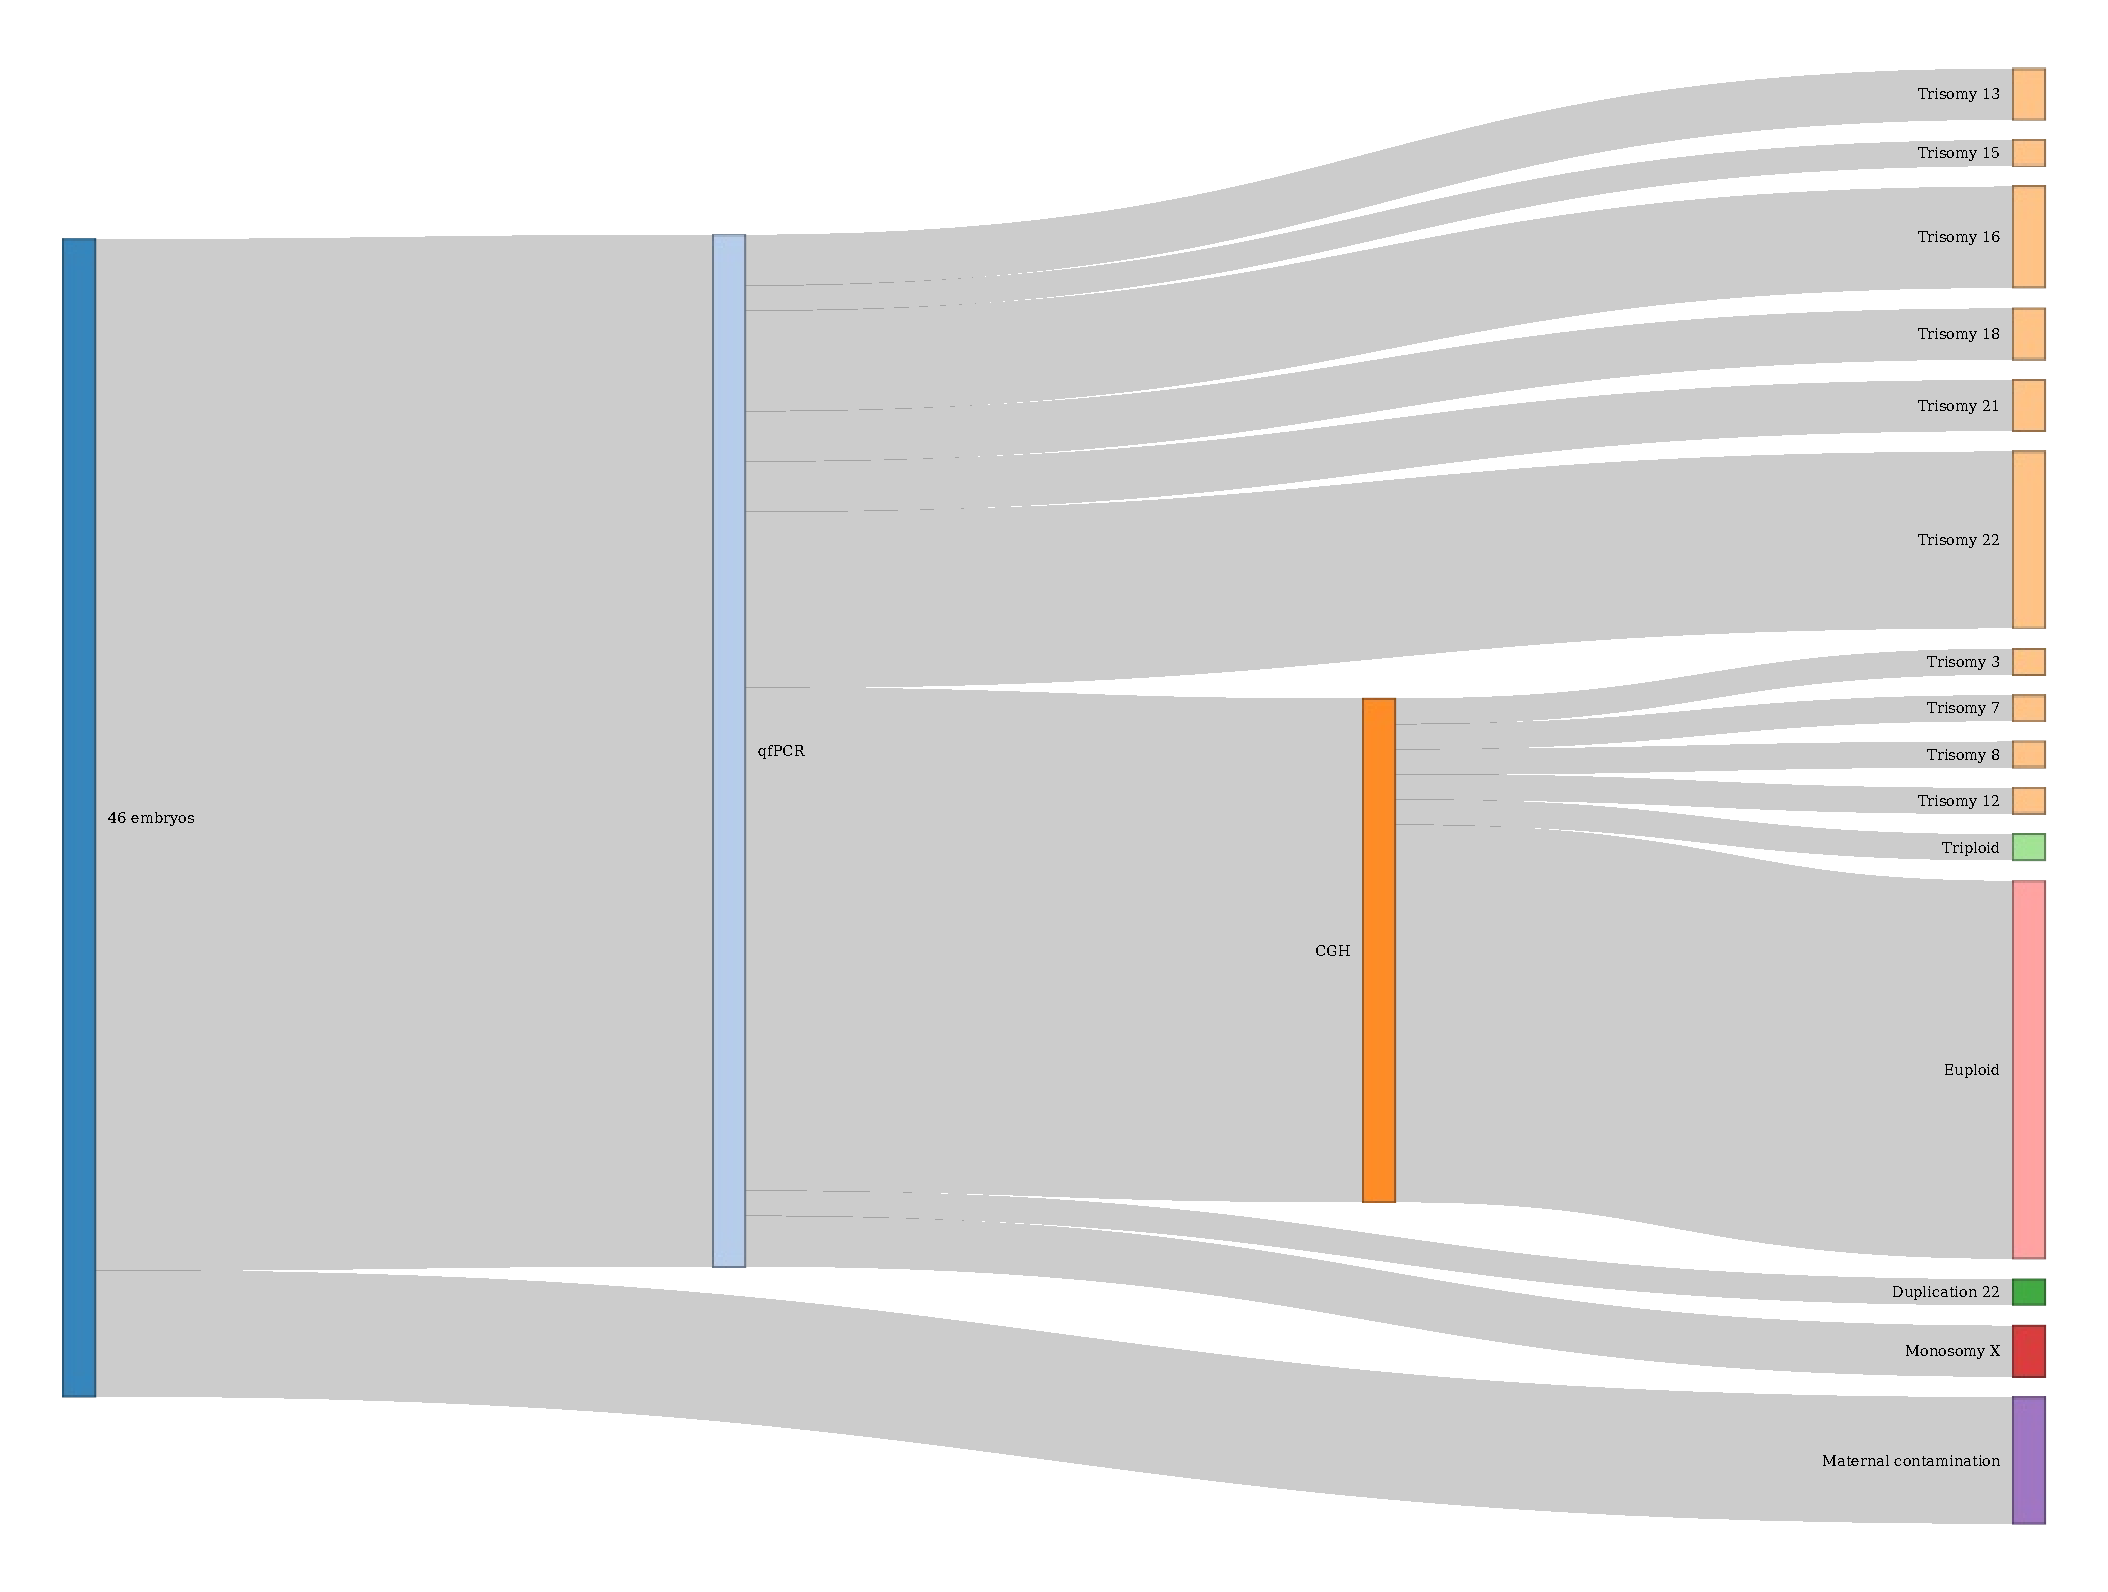
\includegraphics[width=0.7\textwidth]{fig/IbelieveIcanFly.pdf}
\caption{\textbf{Pre-sequencing screening outcome.} }
\label{fig:presequencing}
\end{figure}

\begin{figure}[ht]
\centering
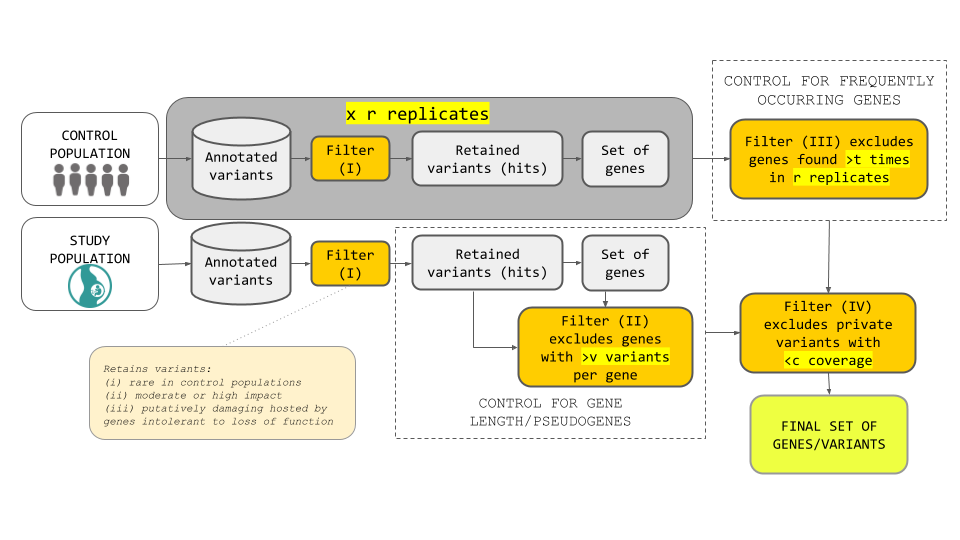
\includegraphics[width=\linewidth]{fig/pipeonly.png}
\caption{\textbf{Overview of the pipeline for prioritization for sequencing (A) Main steps.} Samples are first screened for the quality of DNA and maternal contamination and then analyzed for aneuploidies. \textbf{(B) Outcomes of the pipeline.} We estimate that 18\% of samples goes to sequencing....} 
\label{fig:pipeline}
\end{figure}

\begin{figure}[ht]
\centering
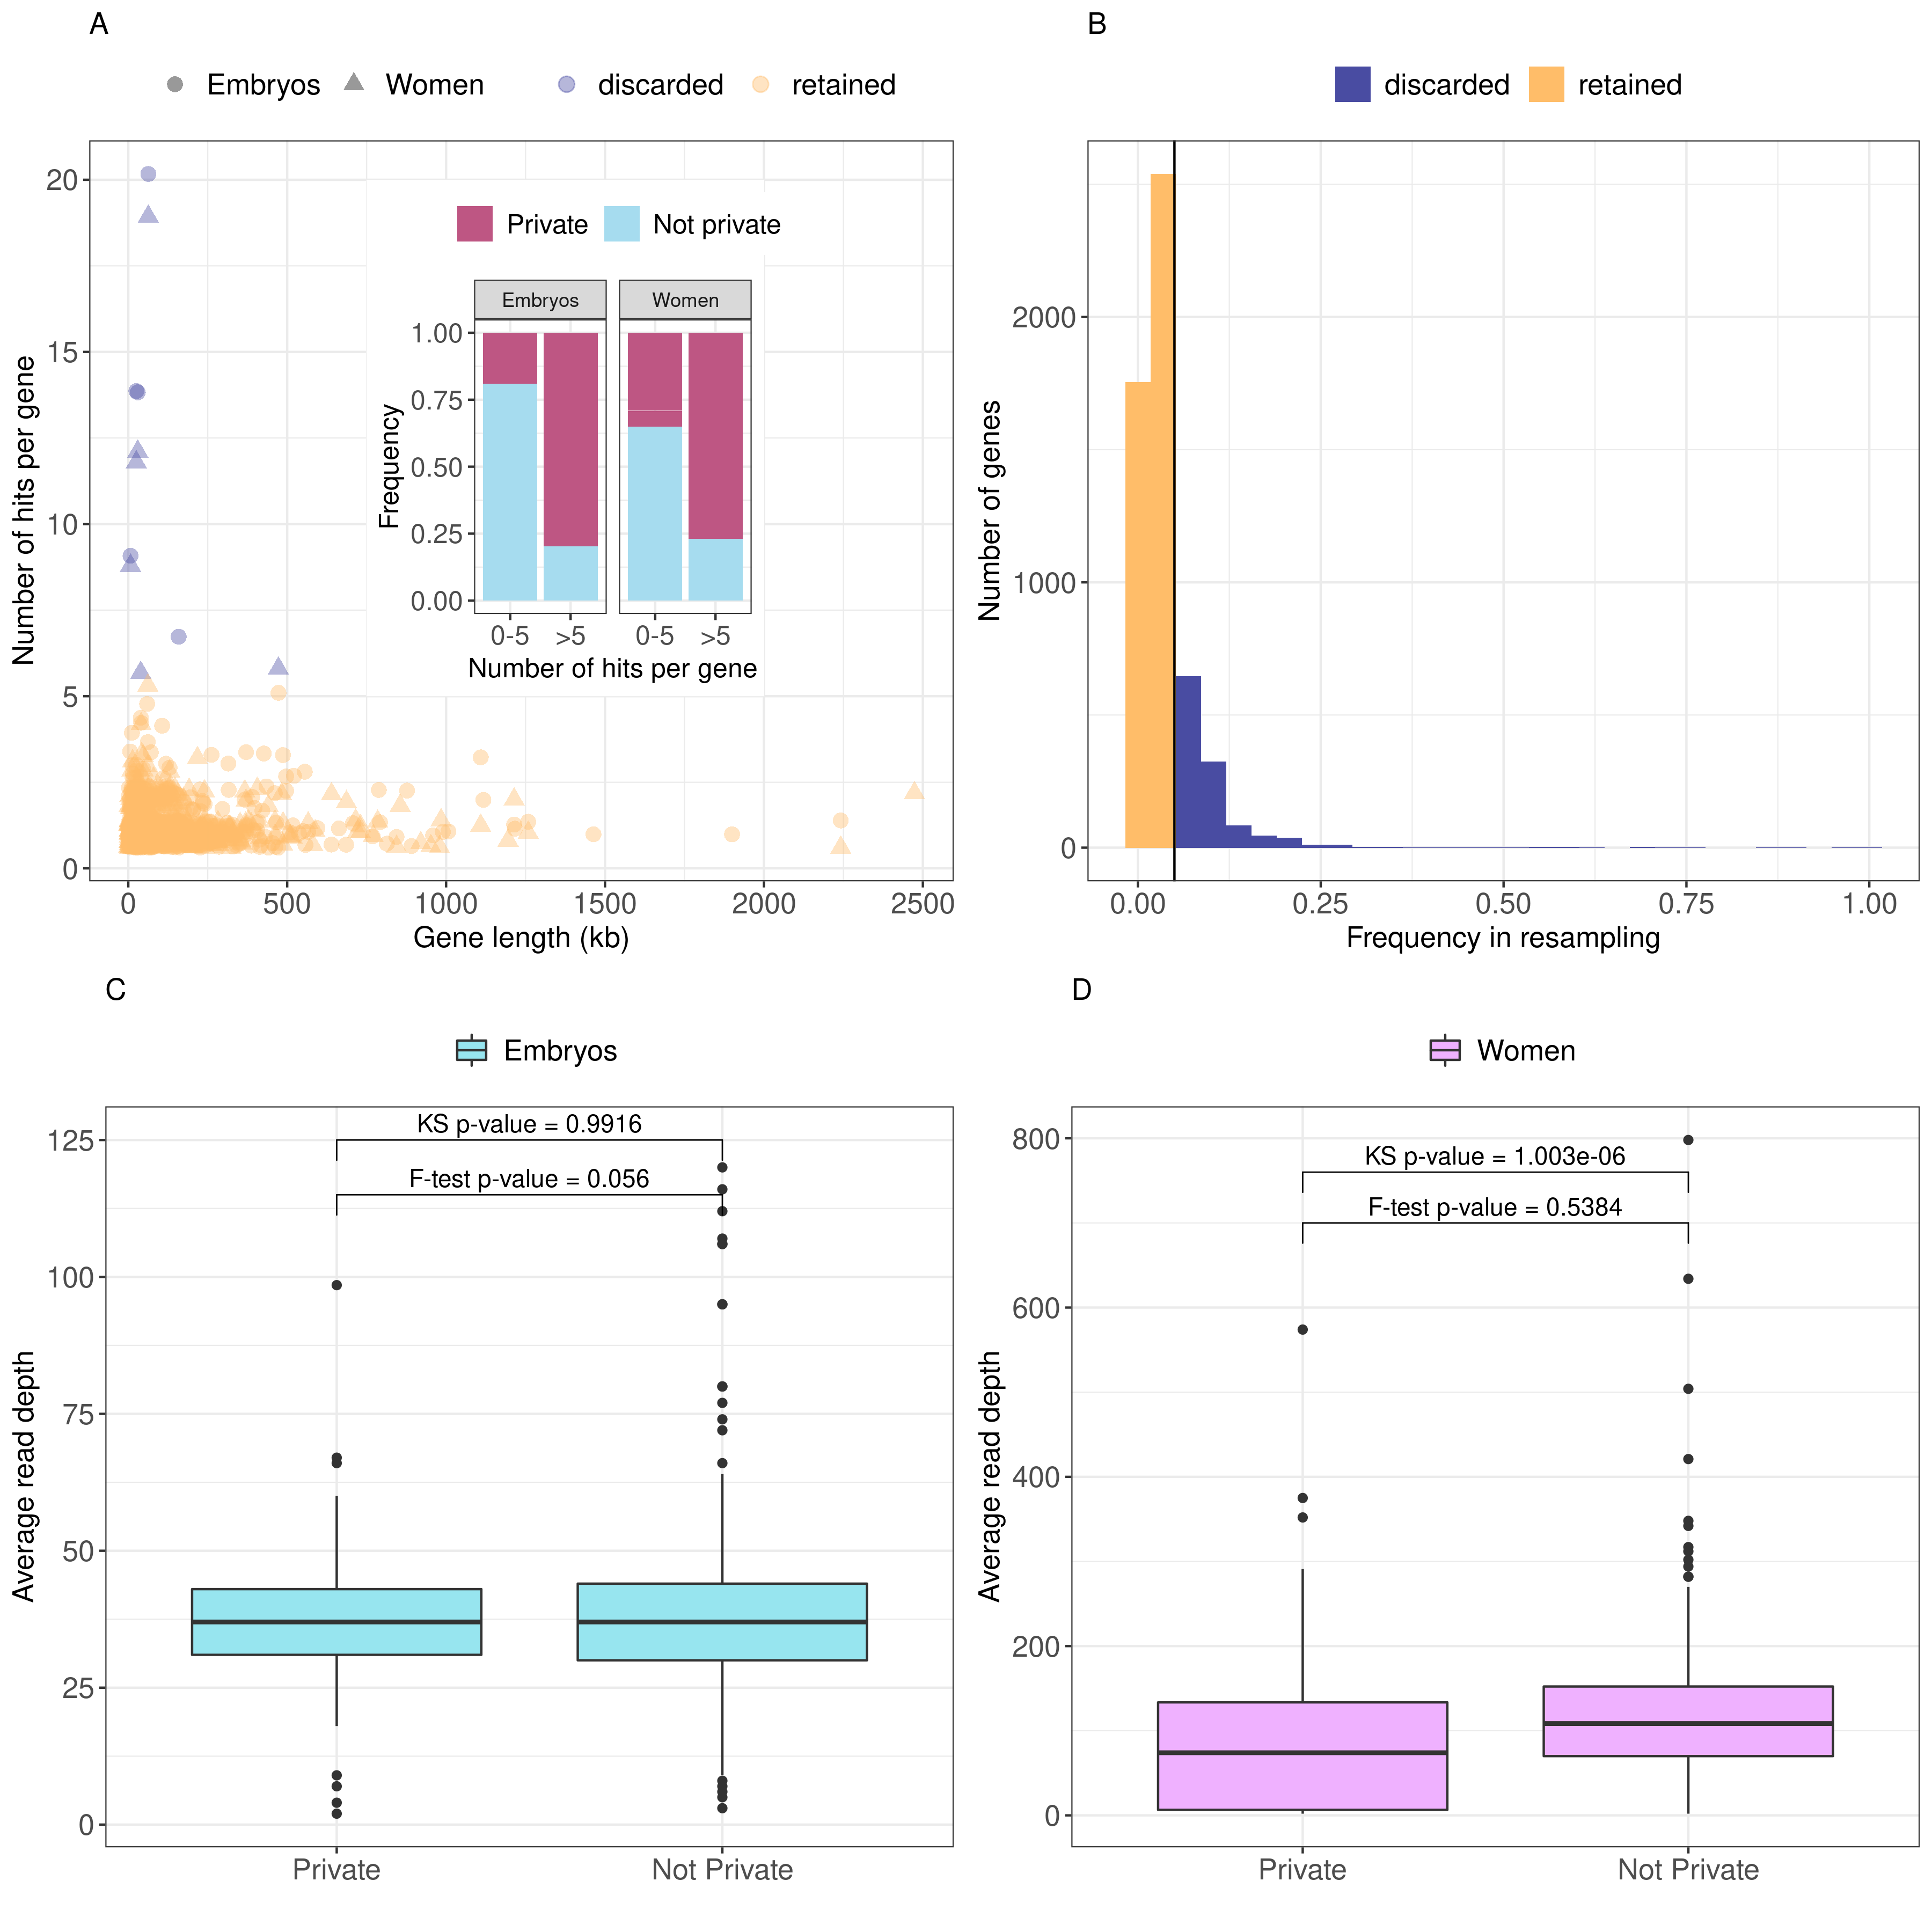
\includegraphics[width=\linewidth]{fig/filters_EmbryoWomen.png}
\caption{\textbf{}}
\label{fig:filters}
\end{figure}

\begin{figure}[ht]
\centering
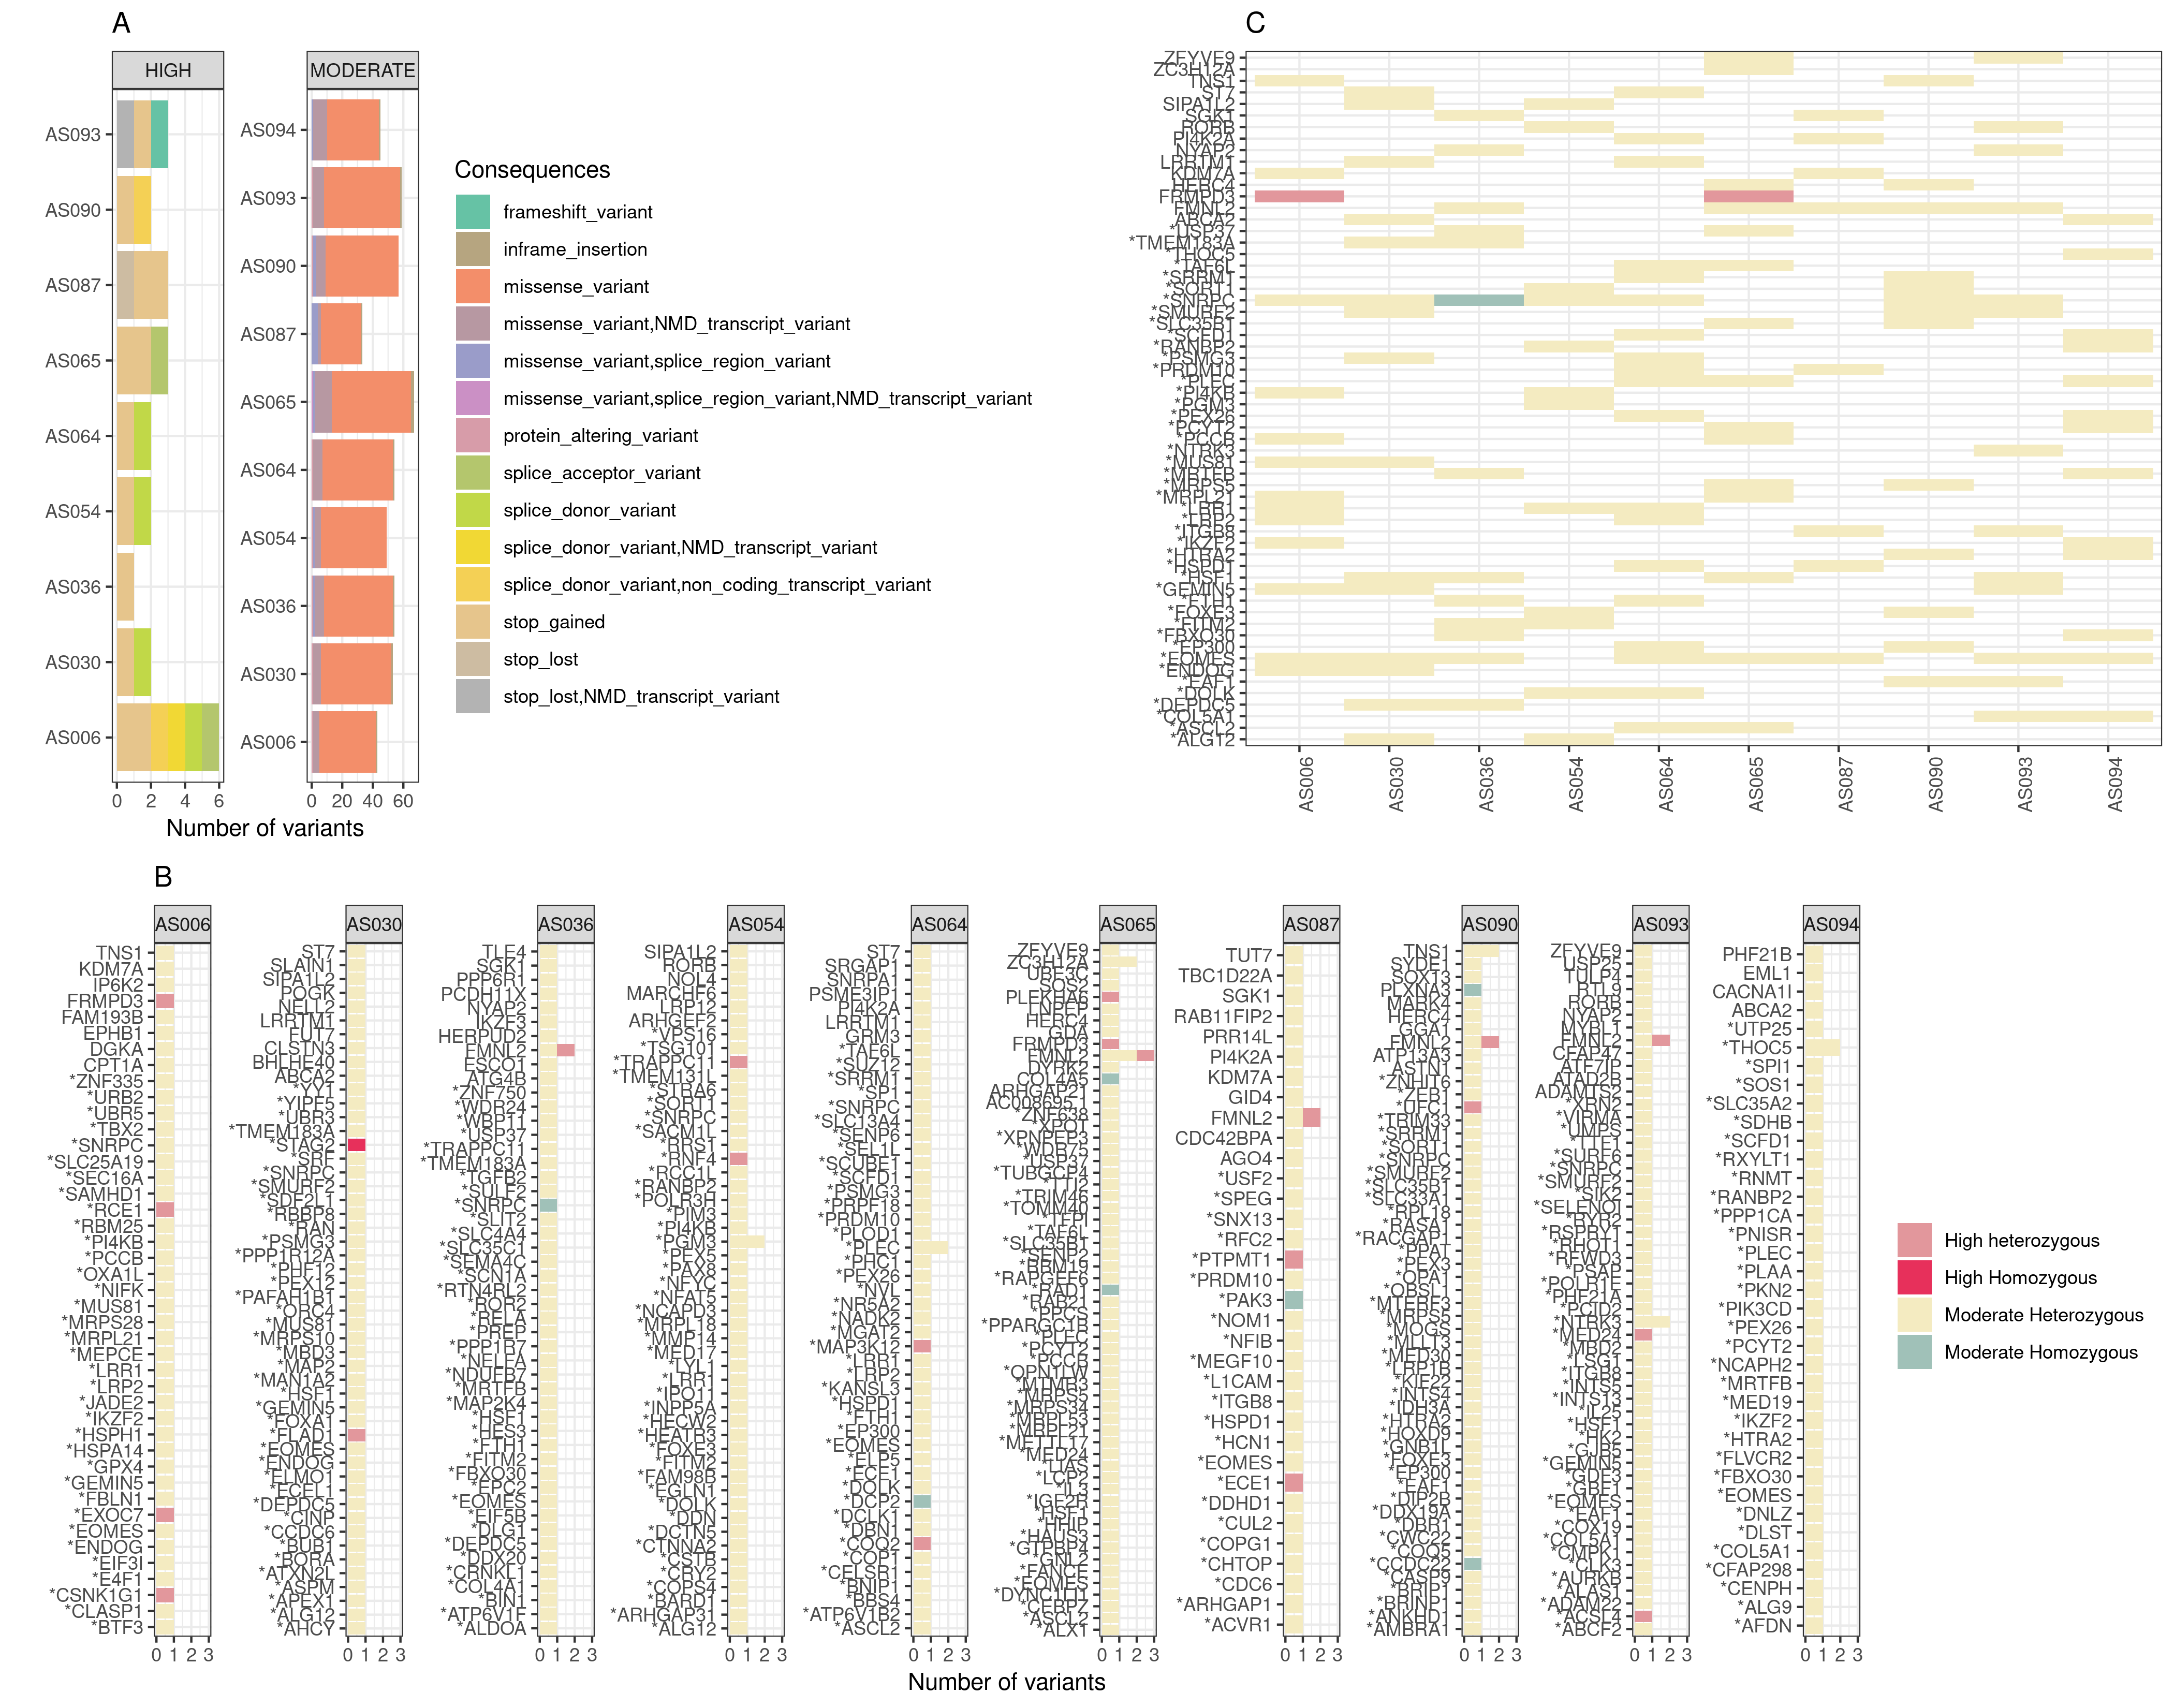
\includegraphics[width=\linewidth]{fig/panel_EmbryoResults.png}
%\caption{\textbf{} he occurrence of variants, their impact, and the count of the consequence allele per gene per embryo  }
\caption{\textbf{}}
\label{fig:resembryo}
\end{figure}

\begin{figure}[ht]
\centering
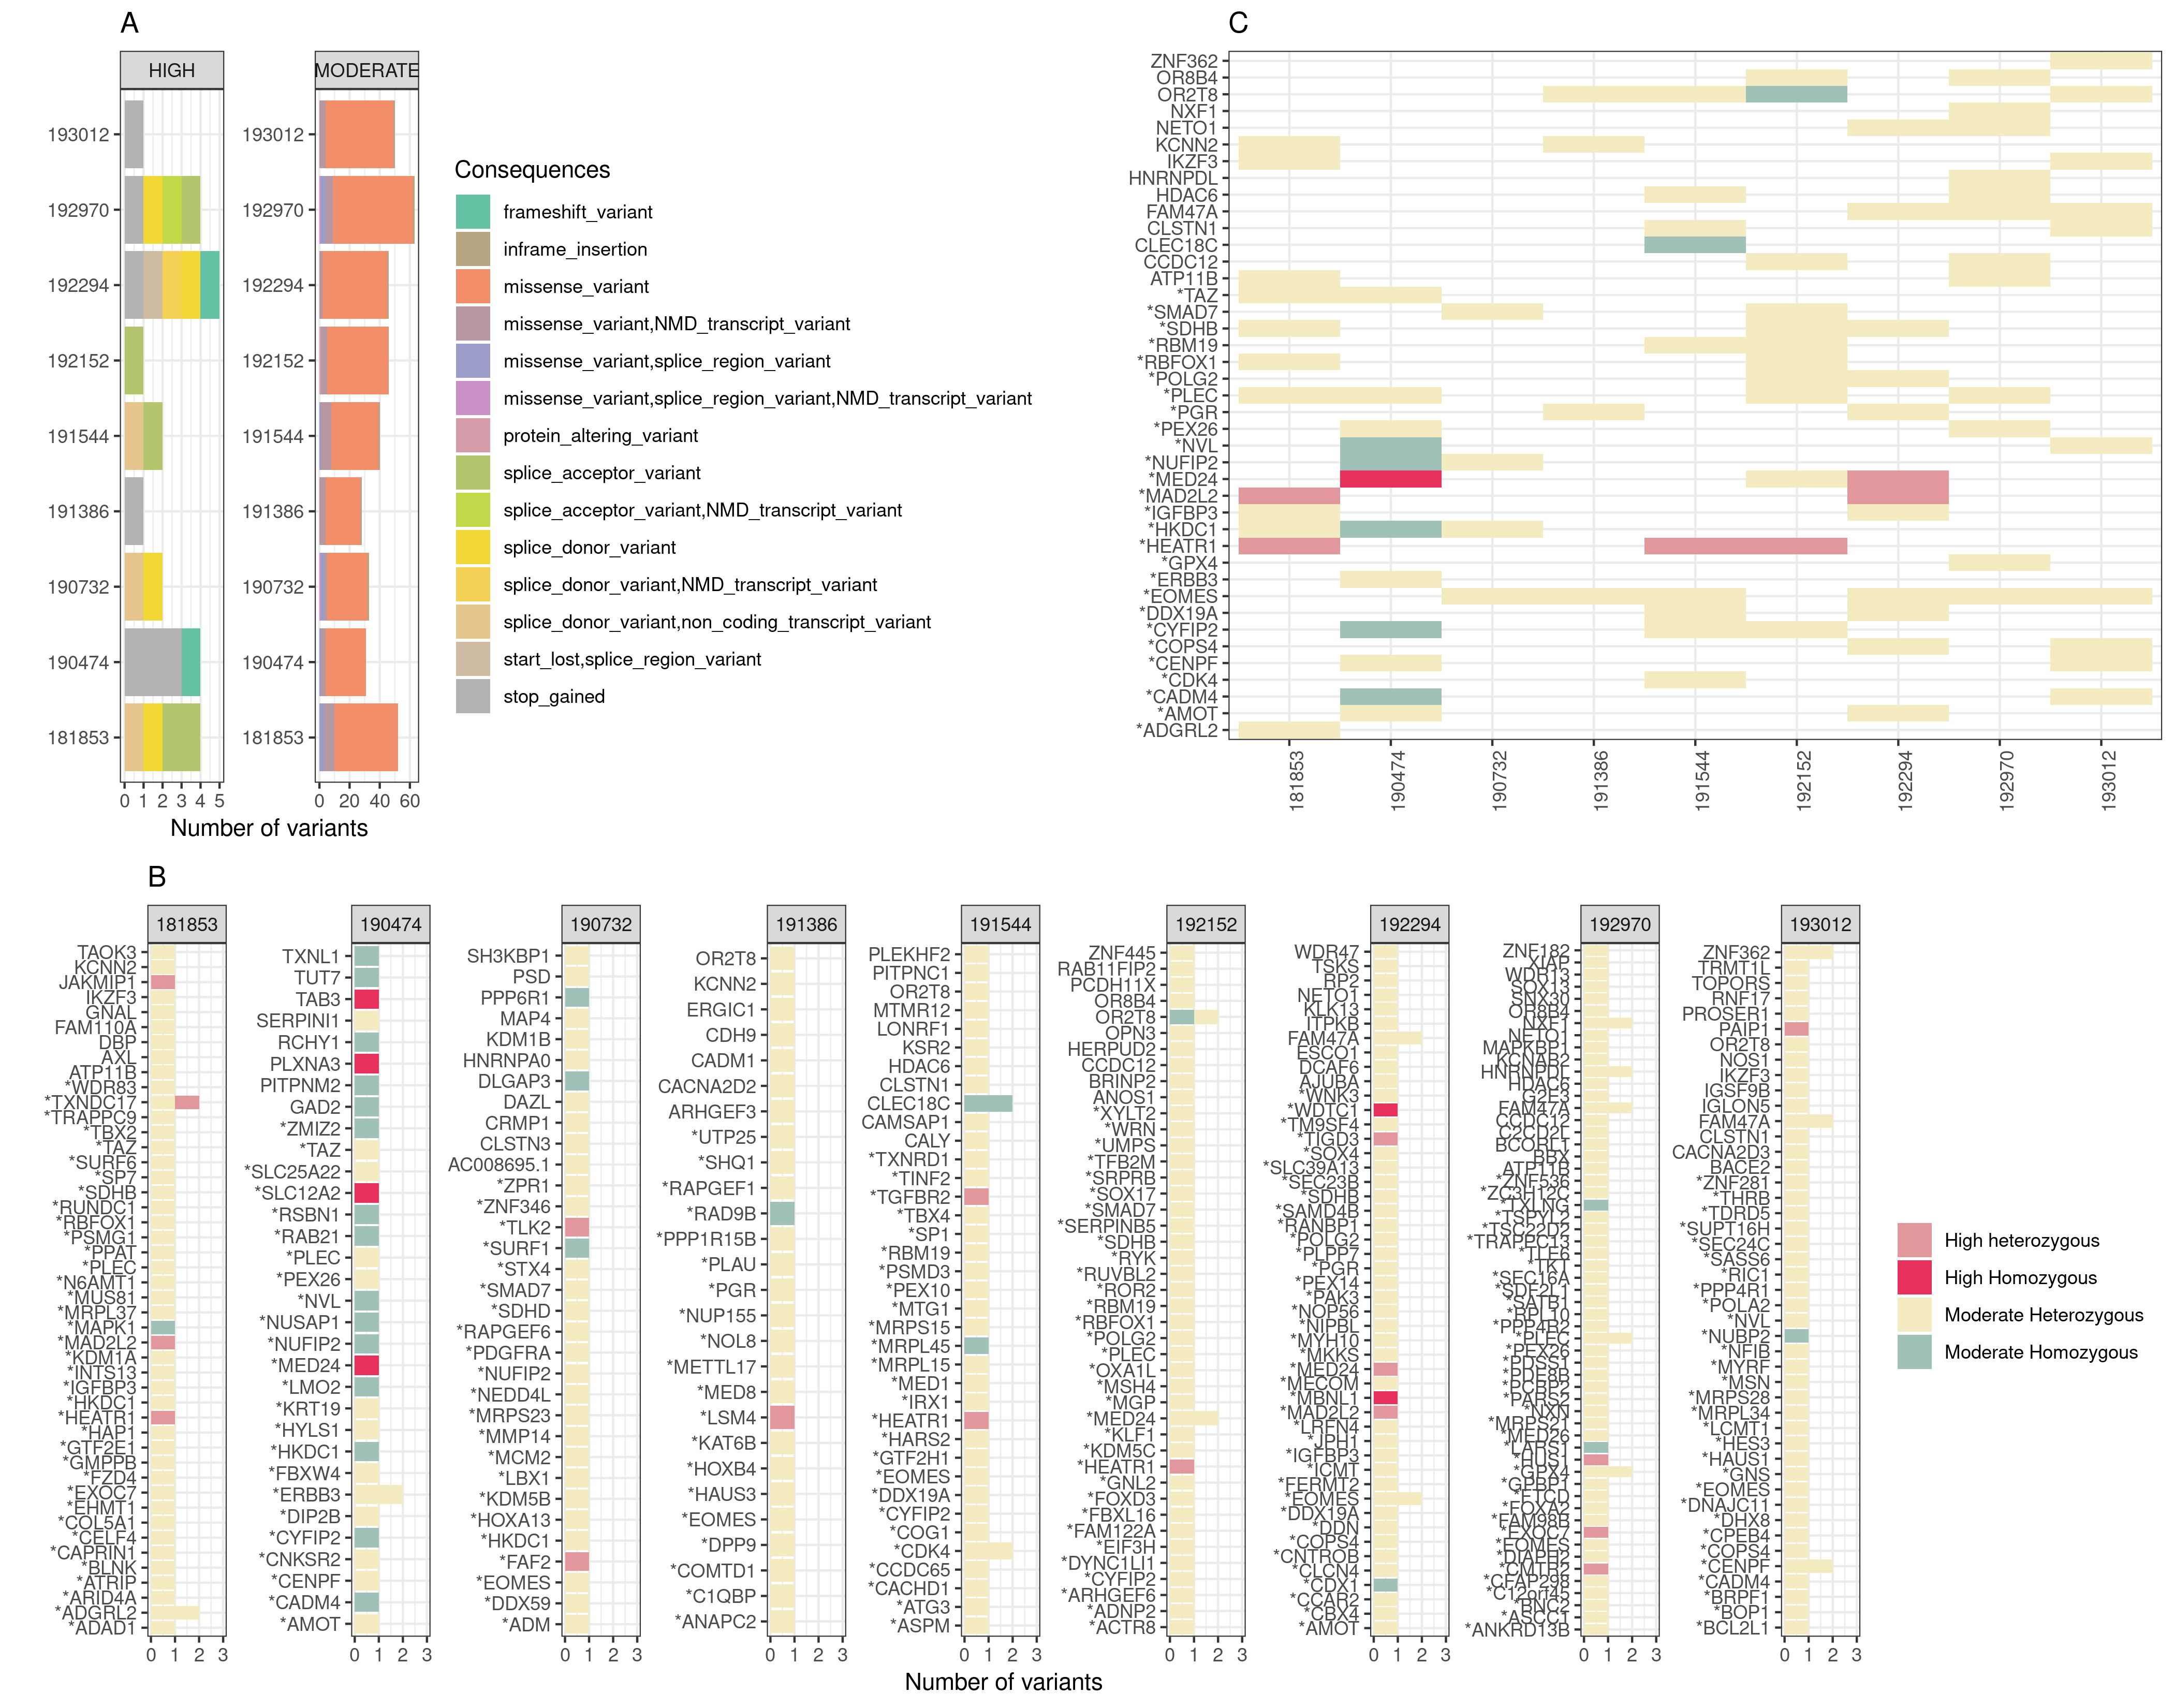
\includegraphics[width=\linewidth]{fig/panel_WomenResults.png}
\caption{\textbf{}  }
\label{fig:reswomen}
\end{figure}



\FloatBarrier

\begin{table}[ht]
\centering
\begin{adjustbox}{width=1\textwidth}
\small
\begin{tabular}{ l c c c c c c c c}
 \hline
 Reactome Term & Pathway	& Total Gene Pathway &	GREP gene & \% expected & Fold Enrichment	& Raw pvalue & FDR \\ [0.5ex]
 \hline
 Activation of RAC1 & R-HSA-428540 &	13	& 4	& .26 & 15.61	& 1.45E-04	& 3.00E-02 \\
 Mitochondrial translation elongation & R-HSA-5389840 &	88	& 9	& 1.73 &	5.19	& 7.87E-05	& 4.49E-02 \\
 Mitochondrial translation termination & R-HSA-5419276 &	88	& 9	& 1.73	& 5.19 &	7.87E-05	& 3.59E-02 \\
 Mitochondrial translation initiation & R-HSA-5368286 &	88	& 9	& 1.73 & 5.19 & 7.87E-05	& 3.00E-02 \\
 Mitochondrial translation & R-HSA-5368287 &	94	& 9	 &1.85 &	4.86	& 1.29E-04	& 2.94E-02 \\
 PPARA activates gene expression & R-HSA-1989781 & 114 &	10 &	2.25 & 4.45	& 1.12E-04	& 3.65E-02 \\
 Regulation of lipid metabolism by PPARalpha & R-HSA-400206 &	115	& 10	& 2.27 & 4.41	& 1.20E-04 & 3.43E-02 \\
 Cell Cycle Checkpoints & R-HSA-69620 &	270 & 16 & 5.32	& 3.01 &	1.22E-04 &	3.09E-02 \\
 Signaling by Rho GTPases & R-HSA-194315 & 417	& 23	& 8.22 &	2.80	& 1.33E-05 & 1.01E-02 \\
%\hline
\caption{This is the caption }
\label{tab:rectomepathways}
\end{tabular}
\end{adjustbox}

\end{table}



\begin{landscape}
\begin{table}[]
\resizebox{\textwidth}{!}{%
\begin{tabular}{|l|l|l|l|l|l|l|l|}
\hline
{\color[HTML]{000000} \textbf{Individual}}      & {\color[HTML]{000000} \textbf{Gene}}            & {\color[HTML]{000000} \textbf{Location}}        & {\color[HTML]{000000} \textbf{Consequence}}       & {\color[HTML]{000000} \textbf{Transcript}} & {\color[HTML]{000000} \textbf{Substitution description}}   & {\color[HTML]{000000} \textbf{SIFT (score)}}             & \textbf{PolyPhen (score)}         \\ \hline
{\color[HTML]{000000} }                         & {\color[HTML]{000000} }                         & {\color[HTML]{000000} }                         & {\color[HTML]{000000} }                           & {\color[HTML]{000000} ENST00000260102}     & {\color[HTML]{000000} c.752G\textgreater{}A, p.Ala237Thr}  & {\color[HTML]{000000} deleterious (0)}                   & deleterious (0)                   \\ \cline{5-8} 
{\color[HTML]{000000} }                         & \multirow{-2}{*}{{\color[HTML]{000000} MRPL15}} & \multirow{-2}{*}{{\color[HTML]{000000} chr 8}}  & \multirow{-2}{*}{{\color[HTML]{000000} missense}} & {\color[HTML]{000000} ENST00000522521}     & {\color[HTML]{000000} c.532G\textgreater{}A, p.Ala178Thr}  & {\color[HTML]{000000} deleterious (0)}                   & deleterious (0)                   \\ \cline{2-8} 
\multirow{-3}{*}{{\color[HTML]{000000} 191544}} & {\color[HTML]{000000} MRPS15}                   & {\color[HTML]{000000} chr 1}                    & {\color[HTML]{000000} missense}                   & {\color[HTML]{000000} ENST00000373116}     & {\color[HTML]{000000} c.864G\textgreater{}A, p.Thr252Ile}  & {\color[HTML]{000000} tolerated (0.1)}                   & tolerated (0.1)                   \\ \hline
{\color[HTML]{000000} }                         & {\color[HTML]{000000} }                         & {\color[HTML]{000000} }                         & {\color[HTML]{000000} }                           & {\color[HTML]{000000} ENST00000276585}     & {\color[HTML]{000000} c.154C\textgreater{}G, p.Arg48Pro}   & {\color[HTML]{000000} tolerated (0.06)}                  & tolerated (0.06)                  \\ \cline{5-8} 
{\color[HTML]{000000} }                         & {\color[HTML]{000000} }                         & {\color[HTML]{000000} }                         & {\color[HTML]{000000} }                           & {\color[HTML]{000000} ENST00000518271}     & {\color[HTML]{000000} c.127C\textgreater{}G, p.Arg43Pro}   & {\color[HTML]{000000} tolerated (0.06)}                  & tolerated (0.06)                  \\ \cline{5-8} 
{\color[HTML]{000000} }                         & \multirow{-3}{*}{{\color[HTML]{000000} MRPS28}} & \multirow{-3}{*}{{\color[HTML]{000000} chr 8}}  & \multirow{-3}{*}{{\color[HTML]{000000} missense}} & {\color[HTML]{000000} ENST00000521605}     & {\color[HTML]{000000} c.184C\textgreater{}G, p.Arg48Pro}   & {\color[HTML]{000000} deleterious (0)}                   & deleterious (0)                   \\ \cline{2-8} 
{\color[HTML]{000000} }                         & {\color[HTML]{000000} }                         & {\color[HTML]{000000} }                         & {\color[HTML]{000000} }                           & {\color[HTML]{000000} ENST00000594999}     & {\color[HTML]{000000} c.351C\textgreater{}T, p.Ala74Val}   & {\color[HTML]{000000} deleterious (0.02)}                & deleterious (0.02)                \\ \cline{5-8} 
{\color[HTML]{000000} }                         & {\color[HTML]{000000} }                         & {\color[HTML]{000000} }                         & {\color[HTML]{000000} }                           & {\color[HTML]{000000} ENST00000595444}     & {\color[HTML]{000000} c.529C\textgreater{}T, p.Ala166Val}  & {\color[HTML]{000000} deleterious low confidence (0.01)} & deleterious low confidence (0.01) \\ \cline{5-8} 
{\color[HTML]{000000} }                         & {\color[HTML]{000000} }                         & {\color[HTML]{000000} }                         & {\color[HTML]{000000} }                           & {\color[HTML]{000000} ENST00000600434}     & {\color[HTML]{000000} c.571C\textgreater{}T, p.Ala74Val}   & {\color[HTML]{000000} deleterious (0.02)}                & deleterious (0.02)                \\ \cline{5-8} 
\multirow{-7}{*}{{\color[HTML]{000000} 193012}} & \multirow{-4}{*}{{\color[HTML]{000000} MRPL34}} & \multirow{-4}{*}{{\color[HTML]{000000} chr 19}} & \multirow{-4}{*}{{\color[HTML]{000000} missense}} & {\color[HTML]{000000} ENST00000252602}     & {\color[HTML]{000000} c.446C\textgreater{}T, p.Ala74Val}   & {\color[HTML]{000000} deleterious (0.02)}                & deleterious (0.02)                \\ \hline
{\color[HTML]{000000} }                         & {\color[HTML]{000000} }                         & {\color[HTML]{000000} }                         & {\color[HTML]{000000} }                           & {\color[HTML]{000000} ENST00000605337}     & {\color[HTML]{000000} c.206C\textgreater{}T, p.Pro53Leu}   & {\color[HTML]{000000} deleterious low confidence (0)}    & deleterious low confidence (0)    \\ \cline{5-8} 
\multirow{-2}{*}{{\color[HTML]{000000} 181853}} & \multirow{-2}{*}{{\color[HTML]{000000} MRPL37}} & \multirow{-2}{*}{{\color[HTML]{000000} chr 1}}  & \multirow{-2}{*}{{\color[HTML]{000000} missense}} & {\color[HTML]{000000} ENST00000360840}     & {\color[HTML]{000000} c.235C\textgreater{}T, p.Pro53Leu}   & {\color[HTML]{000000} deleterious (0)}                   & deleterious (0)                   \\ \hline
{\color[HTML]{000000} }                         & {\color[HTML]{000000} }                         & {\color[HTML]{000000} }                         & {\color[HTML]{000000} }                           & {\color[HTML]{000000} ENST00000581066}     & {\color[HTML]{000000} c.670T\textgreater{}G, p.Leu75Val}   & {\color[HTML]{000000} tolerated (0.28)}                  & tolerated (0.28)                  \\ \cline{5-8} 
\multirow{-2}{*}{{\color[HTML]{000000} 192970}} & \multirow{-2}{*}{{\color[HTML]{000000} MRPS21}} & \multirow{-2}{*}{{\color[HTML]{000000} chr 1}}  & \multirow{-2}{*}{{\color[HTML]{000000} missense}} & {\color[HTML]{000000} ENST00000614145}     & {\color[HTML]{000000} c.434T\textgreater{}G, p.Leu75Val}   & {\color[HTML]{000000} tolerated (0.28)}                  & tolerated (0.28)                  \\ \hline
{\color[HTML]{000000} }                         & {\color[HTML]{000000} }                         & {\color[HTML]{000000} }                         & {\color[HTML]{000000} }                           & {\color[HTML]{000000} ENST00000313608}     & {\color[HTML]{000000} c.210G\textgreater{}T, p.Pro59His}   & {\color[HTML]{000000} tolerated (0.18)}                  & tolerated (0.18)                  \\ \cline{5-8} 
{\color[HTML]{000000} }                         & {\color[HTML]{000000} }                         & {\color[HTML]{000000} }                         & {\color[HTML]{000000} }                           & {\color[HTML]{000000} ENST00000578444}     & {\color[HTML]{000000} c.210G\textgreater{}T, p.Pro59His}   & {\color[HTML]{000000} tolerated (0.12)}                  & tolerated (0.12)                  \\ \cline{5-8} 
\multirow{-3}{*}{{\color[HTML]{000000} 190732}} & \multirow{-3}{*}{{\color[HTML]{000000} MRPS23}} & \multirow{-3}{*}{{\color[HTML]{000000} chr 17}} & \multirow{-3}{*}{{\color[HTML]{000000} missense}} & {\color[HTML]{000000} ENST00000579380}     & {\color[HTML]{000000} c.350G\textgreater{}T, p.Pro7Thr}    & {\color[HTML]{000000} -}                                 & -                                 \\ \hline
{\color[HTML]{000000} }                         & {\color[HTML]{000000} }                         & {\color[HTML]{000000} }                         & {\color[HTML]{000000} }                           & {\color[HTML]{000000} ENST00000285848}     & {\color[HTML]{000000} c.1131G\textgreater{}T, p.Met377Ile} & {\color[HTML]{000000} tolerated (0.51)}                  & tolerated (0.51)                  \\ \cline{5-8} 
{\color[HTML]{000000} }                         & {\color[HTML]{000000} }                         & {\color[HTML]{000000} }                         & {\color[HTML]{000000} }                           & {\color[HTML]{000000} ENST00000358043}     & {\color[HTML]{000000} c.1221G\textgreater{}T, p.Met301Ile} & {\color[HTML]{000000} tolerated (0.33)}                  & tolerated (0.33)                  \\ \cline{5-8} 
{\color[HTML]{000000} }                         & {\color[HTML]{000000} }                         & {\color[HTML]{000000} }                         & {\color[HTML]{000000} }                           & {\color[HTML]{000000} ENST00000412791}     & {\color[HTML]{000000} c.951G\textgreater{}T, p.Met317Ile}  & {\color[HTML]{000000} tolerated (0.37)}                  & tolerated (0.37)                  \\ \cline{5-8} 
\multirow{-4}{*}{{\color[HTML]{000000} 192152}} & \multirow{-4}{*}{{\color[HTML]{000000} OXA1L}}  & \multirow{-4}{*}{{\color[HTML]{000000} chr 14}} & \multirow{-4}{*}{{\color[HTML]{000000} missense}} & {\color[HTML]{000000} ENST00000612549}     & {\color[HTML]{000000} c.965G\textgreater{}T, p.Met317Ile}  & {\color[HTML]{000000} tolerated (0.28)}                  & tolerated (0.28)                  \\ \hline
\end{tabular}%
}
\caption{mito PL}
\label{tab:mito}
\end{table}
\end{landscape}


\begin{landscape}
\begin{table}[]
\resizebox{\textwidth}{!}{%
\begin{tabular}{|l|l|l|l|l|}
\hline
{\color[HTML]{000000} \textbf{rs identifier}} & \textbf{genomic location (GRCh38)} & \textbf{HGVS Names}  & \textbf{Functional annotations}                        & \textbf{Alternate allele frequency}\\ \hline
{\color[HTML]{000000} rs866373641}  & chr2 152560918  & c.479G\textgreater{}T, p.Ser160Ile  & missense, tolerated (SIFT=0.14), benign(PolyPhen=0.02) & 1000G=1\%, gnomADe=1\%, gnomADg=8\%, TOPMed=18\% \\ \hline
{\color[HTML]{000000} rs750755379} & chr2 152560914 & c.475G\textgreater{}T,  p.Glu159Ter & stop gain & 1000G=1\%, gnomADe=1.3\%, gnomADg=10.3\%, TOPMed=25.3\% \\ \hline
\end{tabular}%
}
\caption{\textit{FMNL2} TT haplotype - HGVS - Human Genome Variation Society}
\label{tab:fmnl2}
\end{table}
\end{landscape}

\beginsupplement
\section*{Supplementary Information}
%%%%%%%%%%%%%%%%%%%%%%%%%
\subsection*{Supplementary Tables}
\begin{landscape}
\begin{table}[]
\resizebox{\textwidth}{!}{%
\begin{tabular}{|l|l|l|l|l|l|l|}
\hline
{\color[HTML]{000000} \textbf{ID}} & \textbf{origin} & \textbf{Full term births} & \textbf{Previous miscarriages} & \textbf{Induced abortion} & \textbf{Preterm birth} & \textbf{type of miscarriage} \\ \hline
{\color[HTML]{000000} AS006}       & European        & 0                         & 0                              & 0                         & 0                      & miscarriage first            \\ \hline
{\color[HTML]{000000} AS030}       & European        & 1                         & 1                              & 0                         & 0                      & miscarriage first            \\ \hline
AS036                              & European        & 0                         & 0                              & 0                         & 0                      & miscarriage first            \\ \hline
AS054                              & African         & 1                         & 0                              & 2                         & 0                      & miscarriage first            \\ \hline
AS064                              & European        & 0                         & 0                              & 0                         & 0                      & miscarriage\_first           \\ \hline
AS065                              & European        & 0                         & 0                              & 0                         & 0                      & miscarriage first            \\ \hline
AS087                              & Asian           & 0                         & 3                              & 0                         & 1                      & miscarriage recurrent        \\ \hline
AS090                              & European        & 1                         & 0                              & 0                         & 0                      & miscarriage first            \\ \hline
AS093                              & Asian           & 0                         & 2                              & 0                         & 0                      & miscarriage recurrent        \\ \hline
AS094                              & European        & 3                         & 3                              & 0                         & 0                      & miscarriage recurrent        \\ \hline
\end{tabular}%
}
\caption{}
\label{tab:medicalfields}
\end{table}
\end{landscape}

\begin{landscape}
\begin{table}[]
\resizebox{\textwidth}{!}{%
\begin{tabular}{|l|l|l|l|l|}
\hline
\textbf{Gene symbol} & \textbf{Gene length (kb)} & \textbf{Nb. of paralogues (range identity)} & \textbf{hist in embryos} & \textbf{hits in women} \\ \hline
\textit{C2CD3}       & 7.96                      &                                             & 7                        & 0                      \\ \hline
\textit{FIGN}        & 9.5                       & 10 (24-41\%)                                & 16                       & 0                      \\ \hline
\textit{GXYLT1}      & 63                        &                                             & 20                       & 19                     \\ \hline
\textit{MTCH2}       & 29.8                      &                                             & 14                       & 12                     \\ \hline
\textit{MUC1}        & 7.09                      &                                             & 9                        & 9                      \\ \hline
\textit{MUC5B}       & 39.1                      &                                             & 0                        & 6                      \\ \hline
\textit{PCSK5}       & 472                       & 9 (11-52\%)                                 & 0                        & 6                      \\ \hline
\end{tabular}%
}
\caption{Caption}
\label{tab:paralogs}
\end{table}
\end{landscape}


%%%%%%%%%%%%%%%%%%%%%%%%%%
\subsection*{Supplementary Figures}
\begin{figure}[ht]
\centering
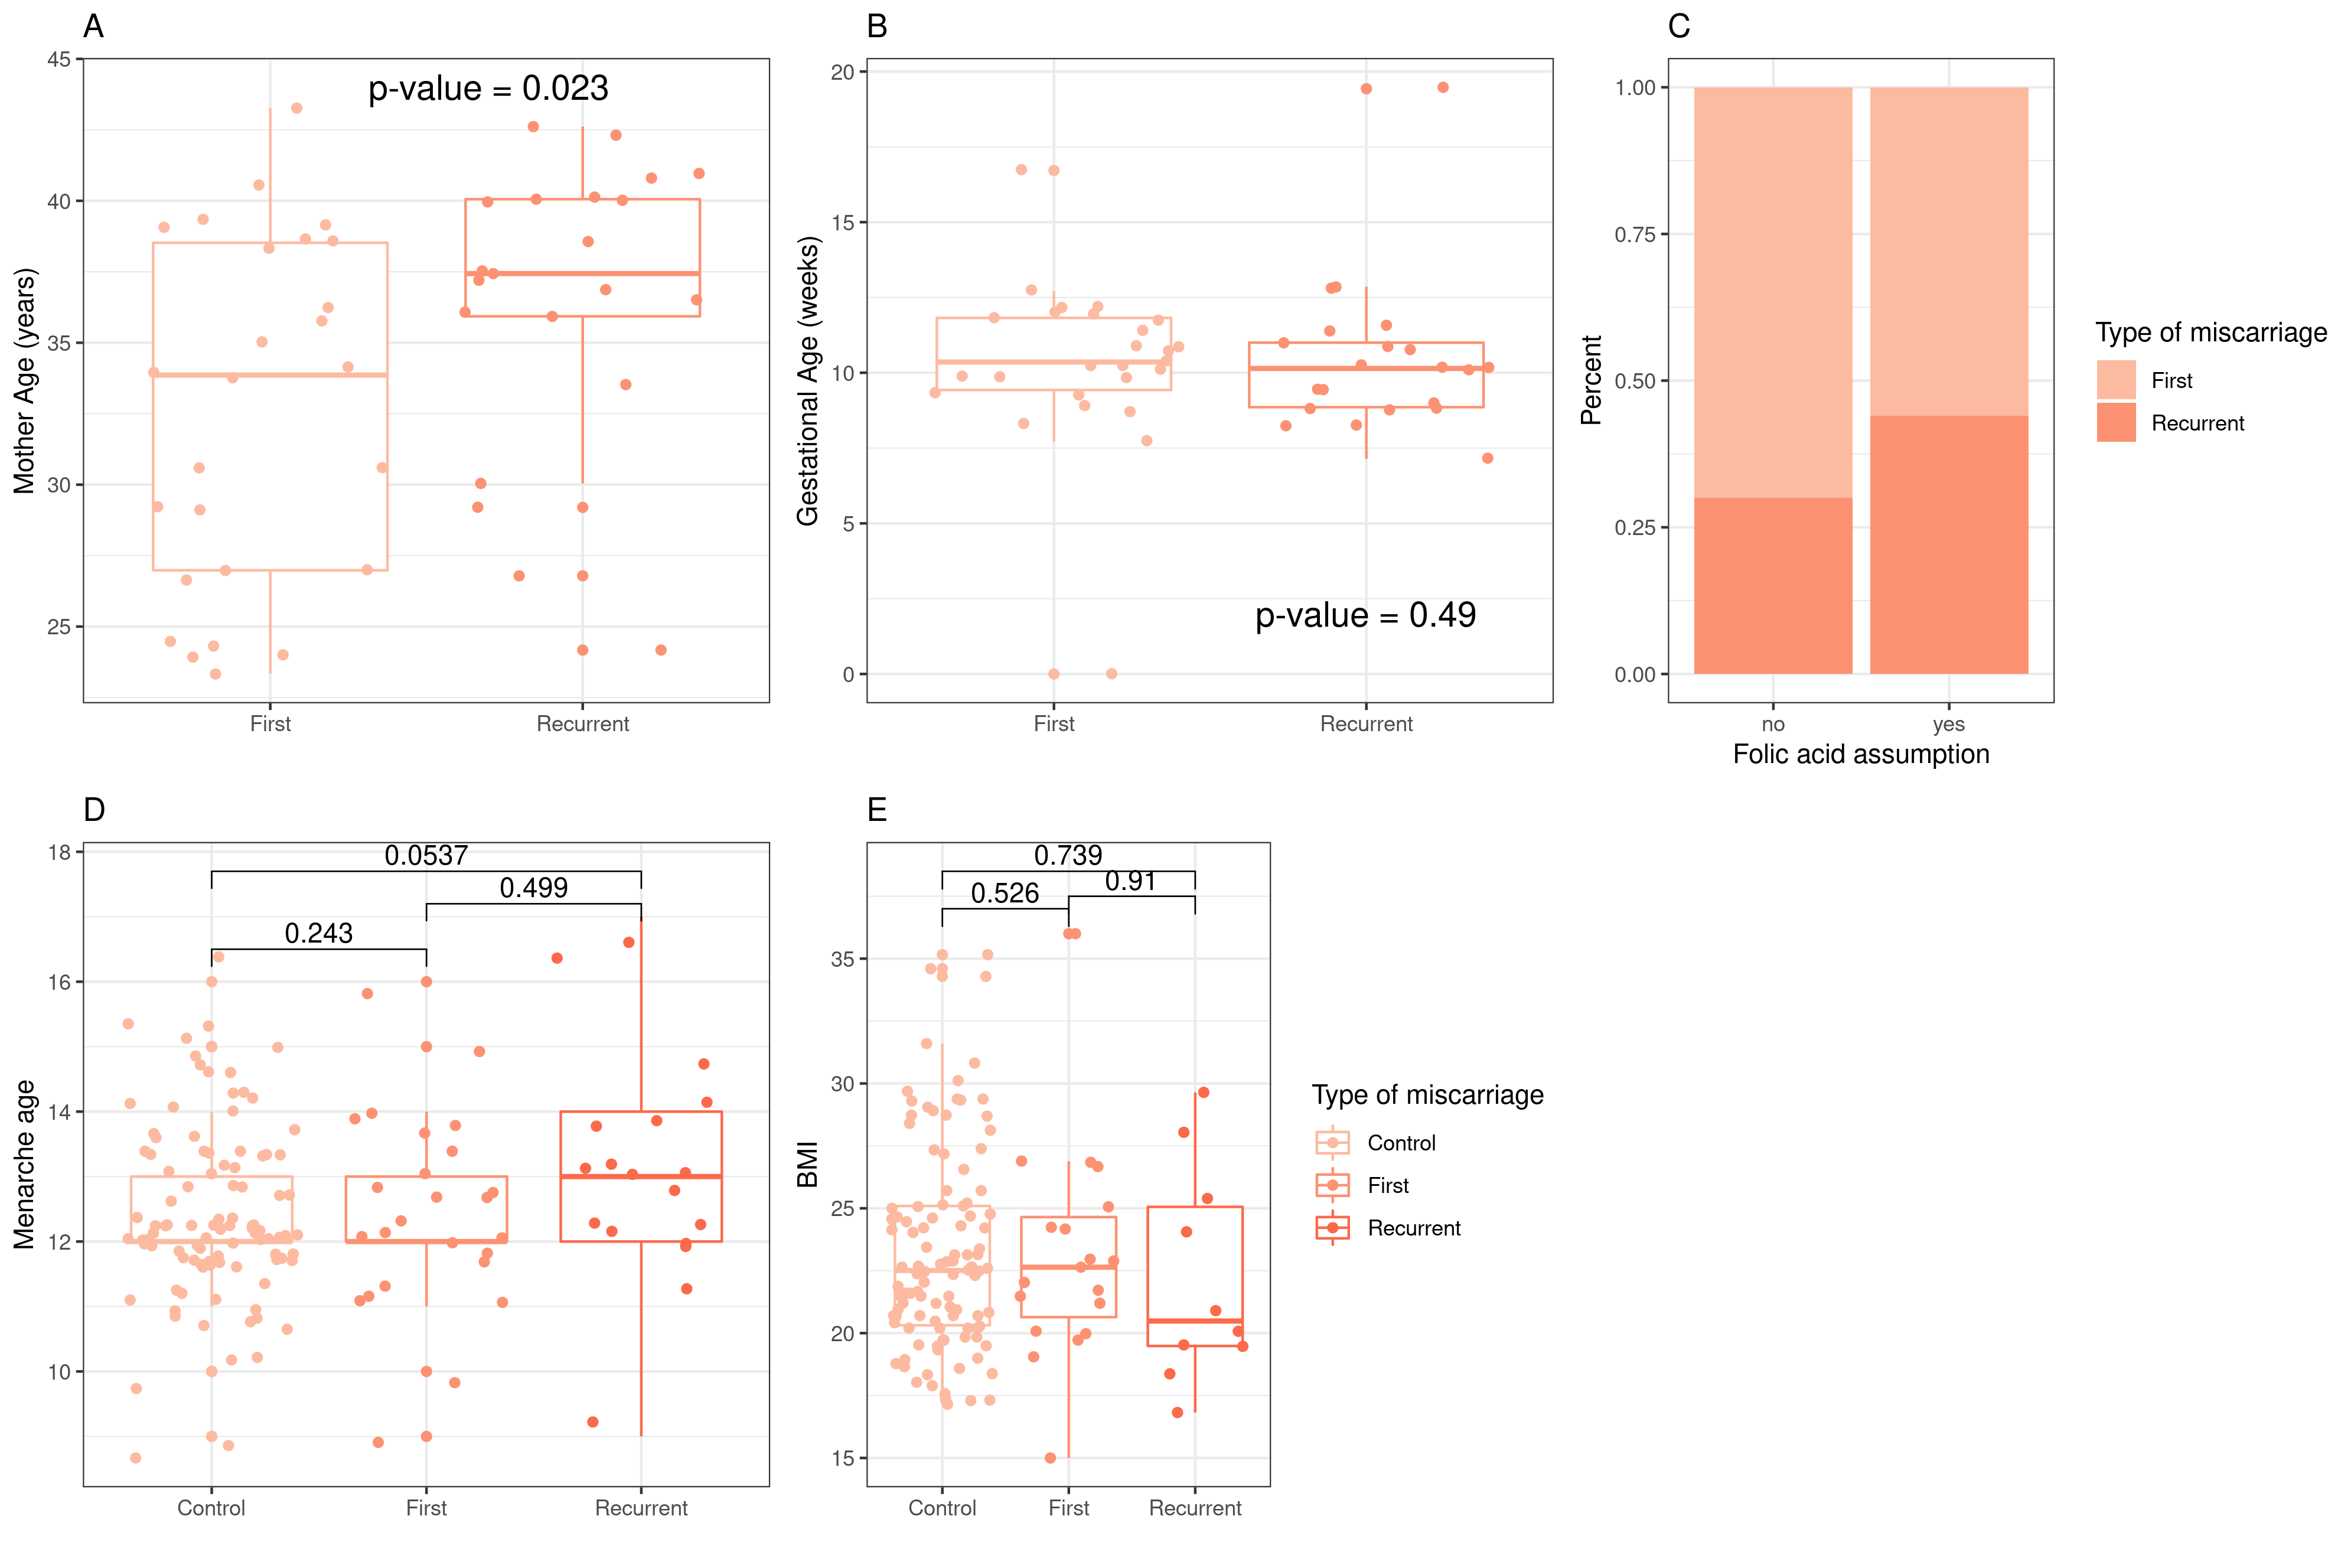
\includegraphics[width=\linewidth]{fig/panel_stats.png}
\caption{\textbf{Features of the embryo's mothers.} \textbf{(A)} Median age of the mother at the event is XX and XX for first and recurrent miscarriages, with no significant difference. \textbf{(B)} Gestational age at the time of the pregnancy termination range from X to X weeks with no significant difference between first and recurrent cases.  \textbf{(C)} Folic acid intake. Range of values of menarche age \textbf{(D)} and Body Mass Index \textbf{(E)} in embryo's mothers are not significantly different from a control set of mothers undergoing voluntary termination of pregnancy.}
\label{fig:embryostats}
\end{figure}

\begin{figure}[ht]
    \centering
    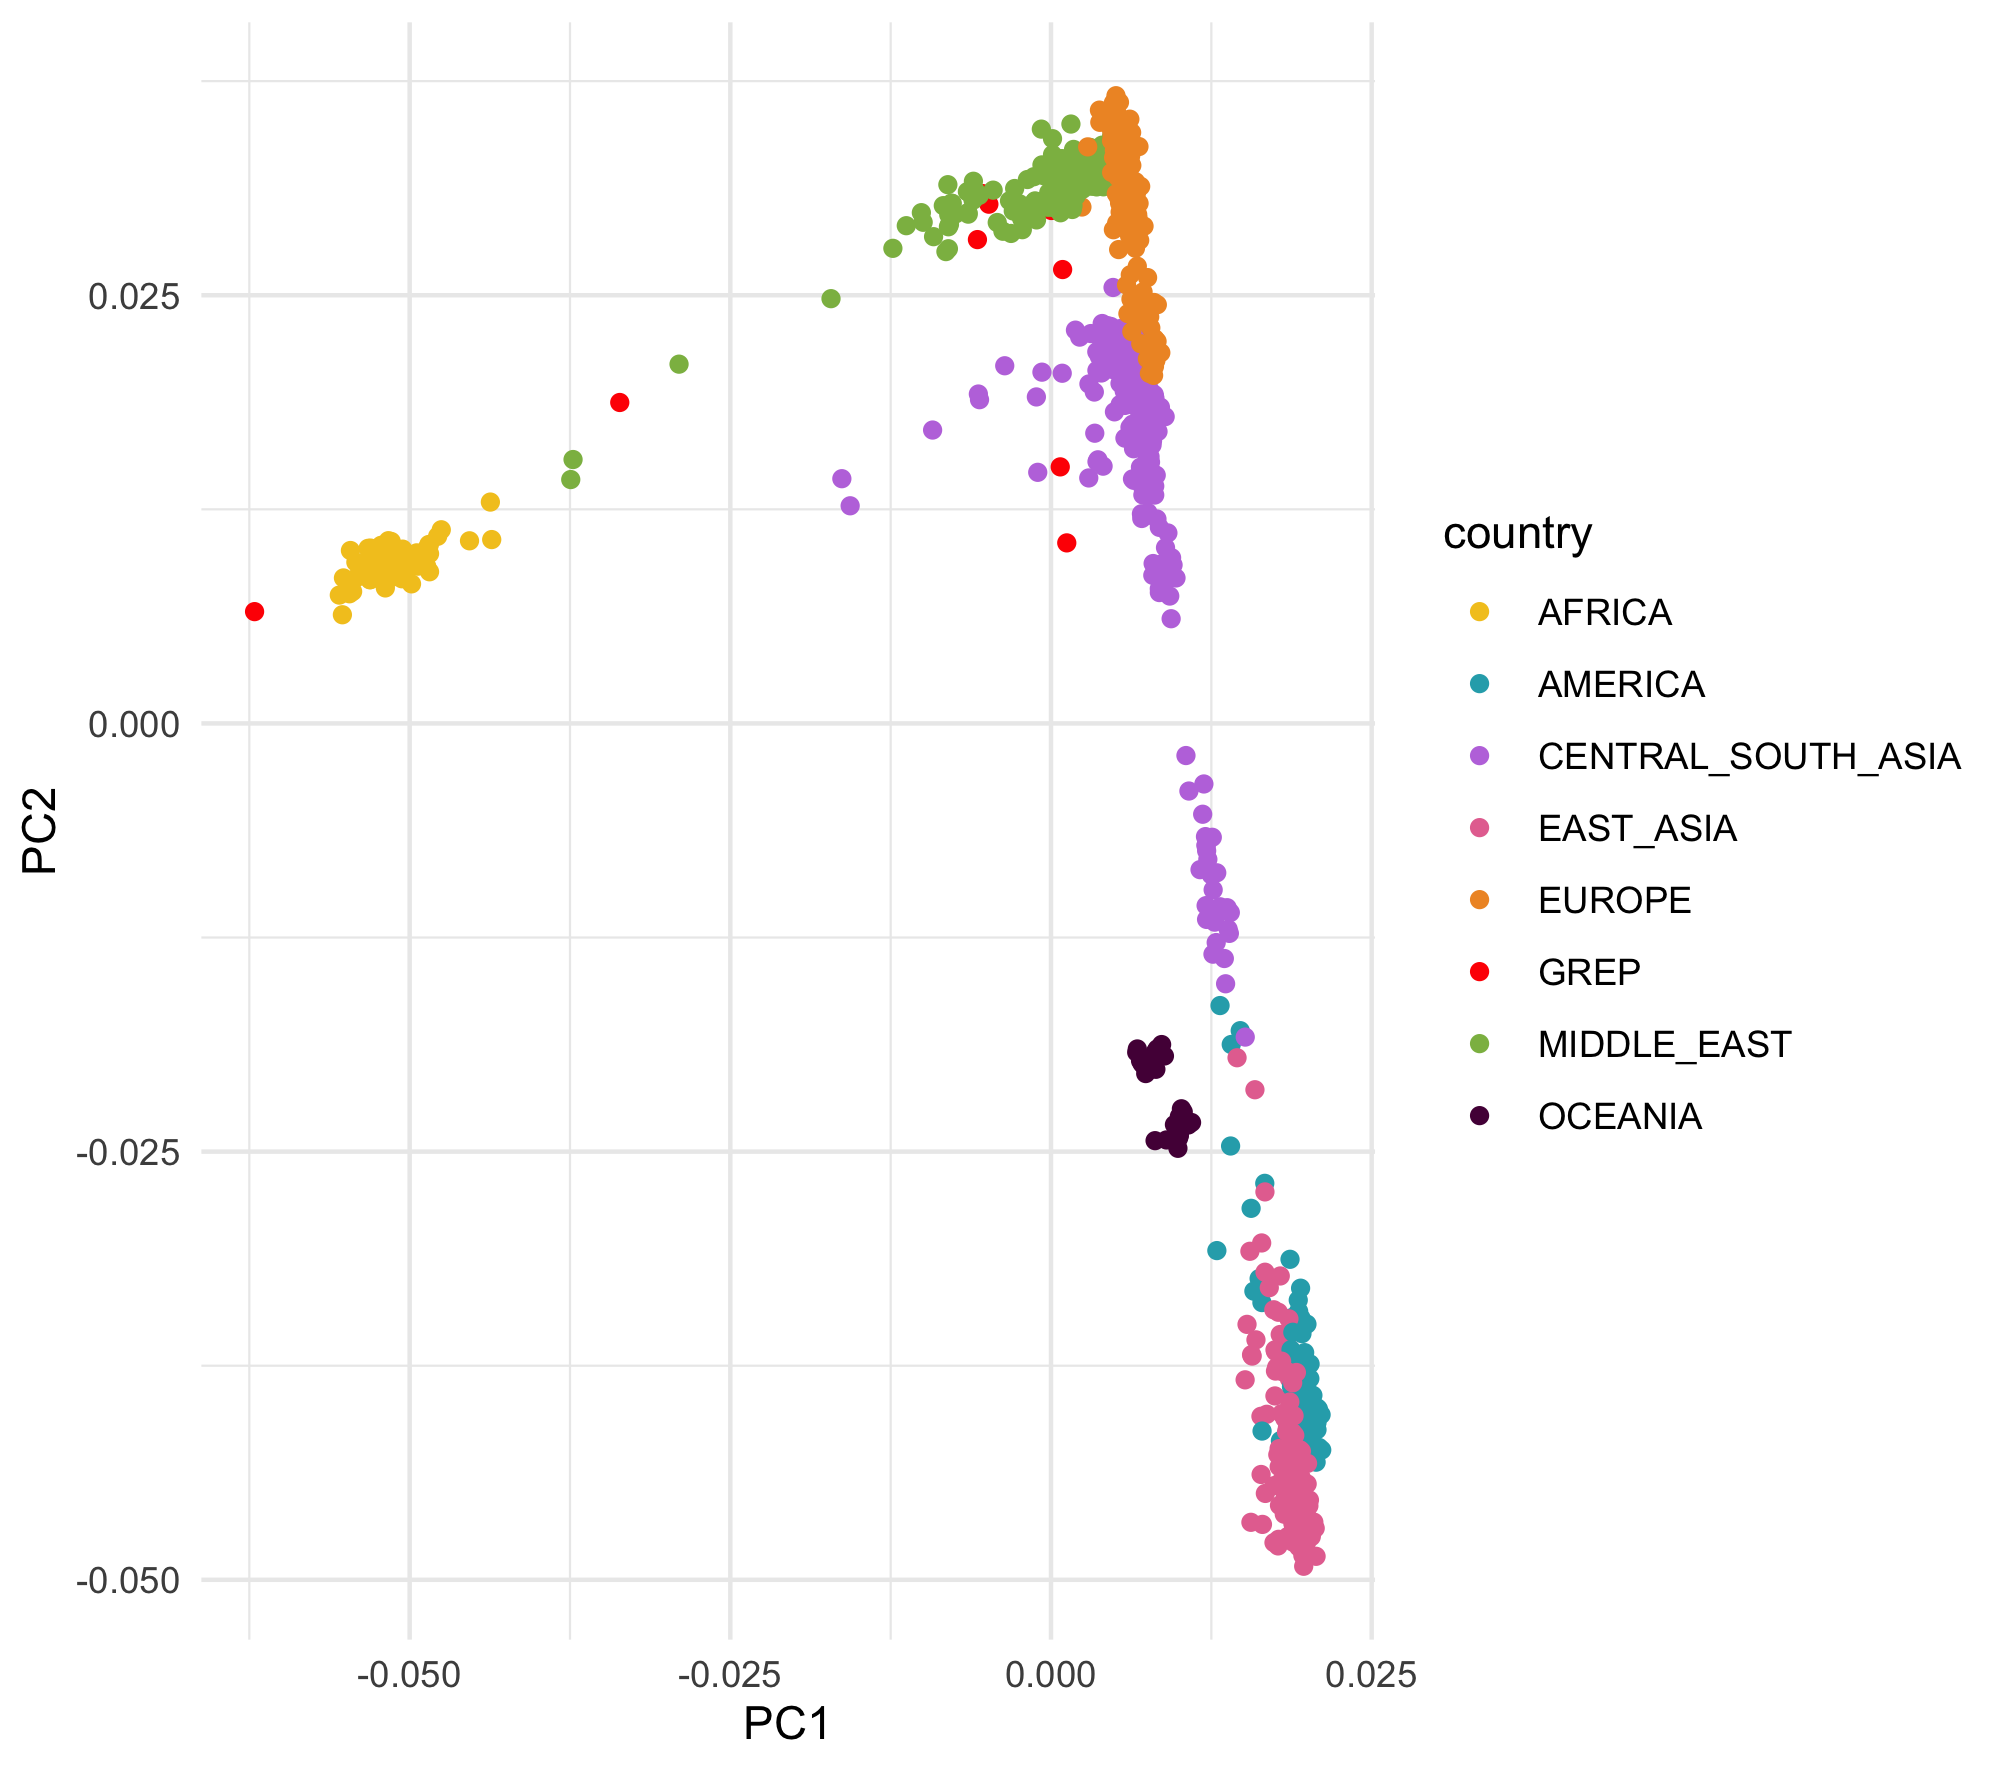
\includegraphics[width= 14 cm, high= 16cm]{fig/pca_hgdp-grep_noALPHA.png}
    \caption{\textbf{Principal Component Analysis  }}
    \label{fig:pca}
\end{figure}


\begin{figure}[ht]
    \centering
    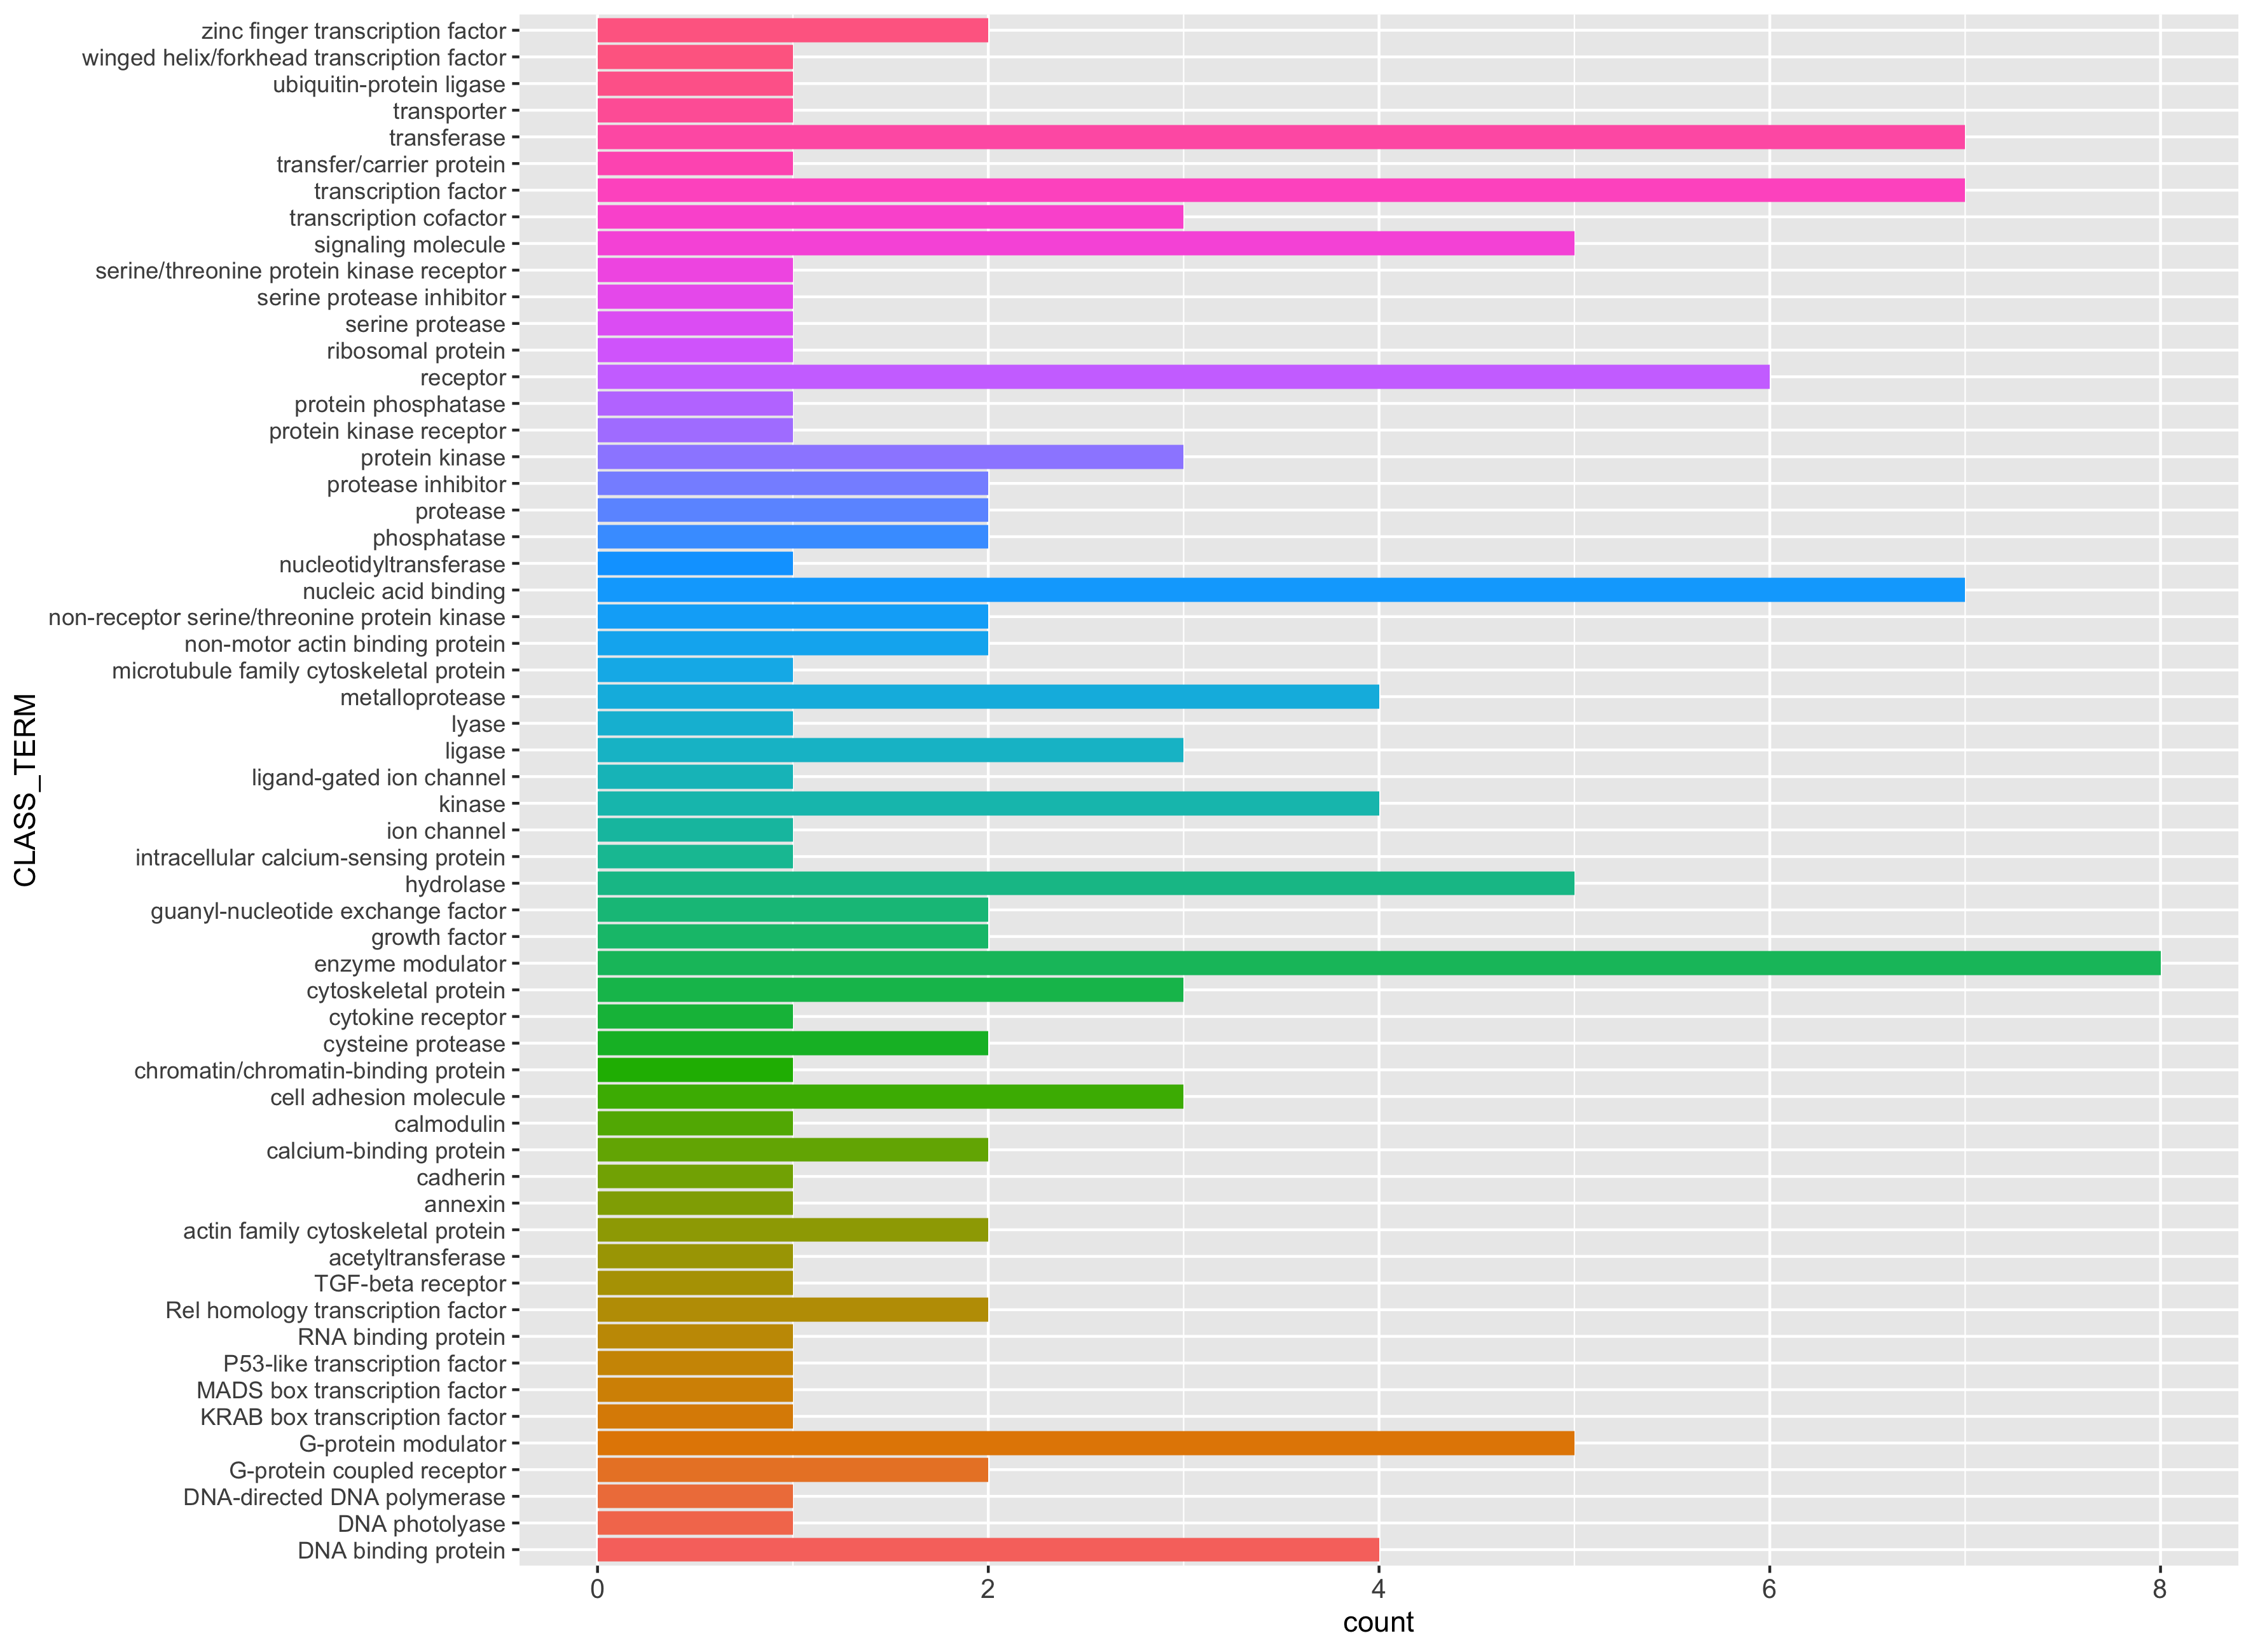
\includegraphics[width= 14 cm, high= 16cm]{fig/class_term_grep.png}
    \caption{\textbf{Classification of the prioritized genes by protein class. }}
    \label{fig:protClass}
\end{figure}


\begin{figure}[ht]
    \centering
    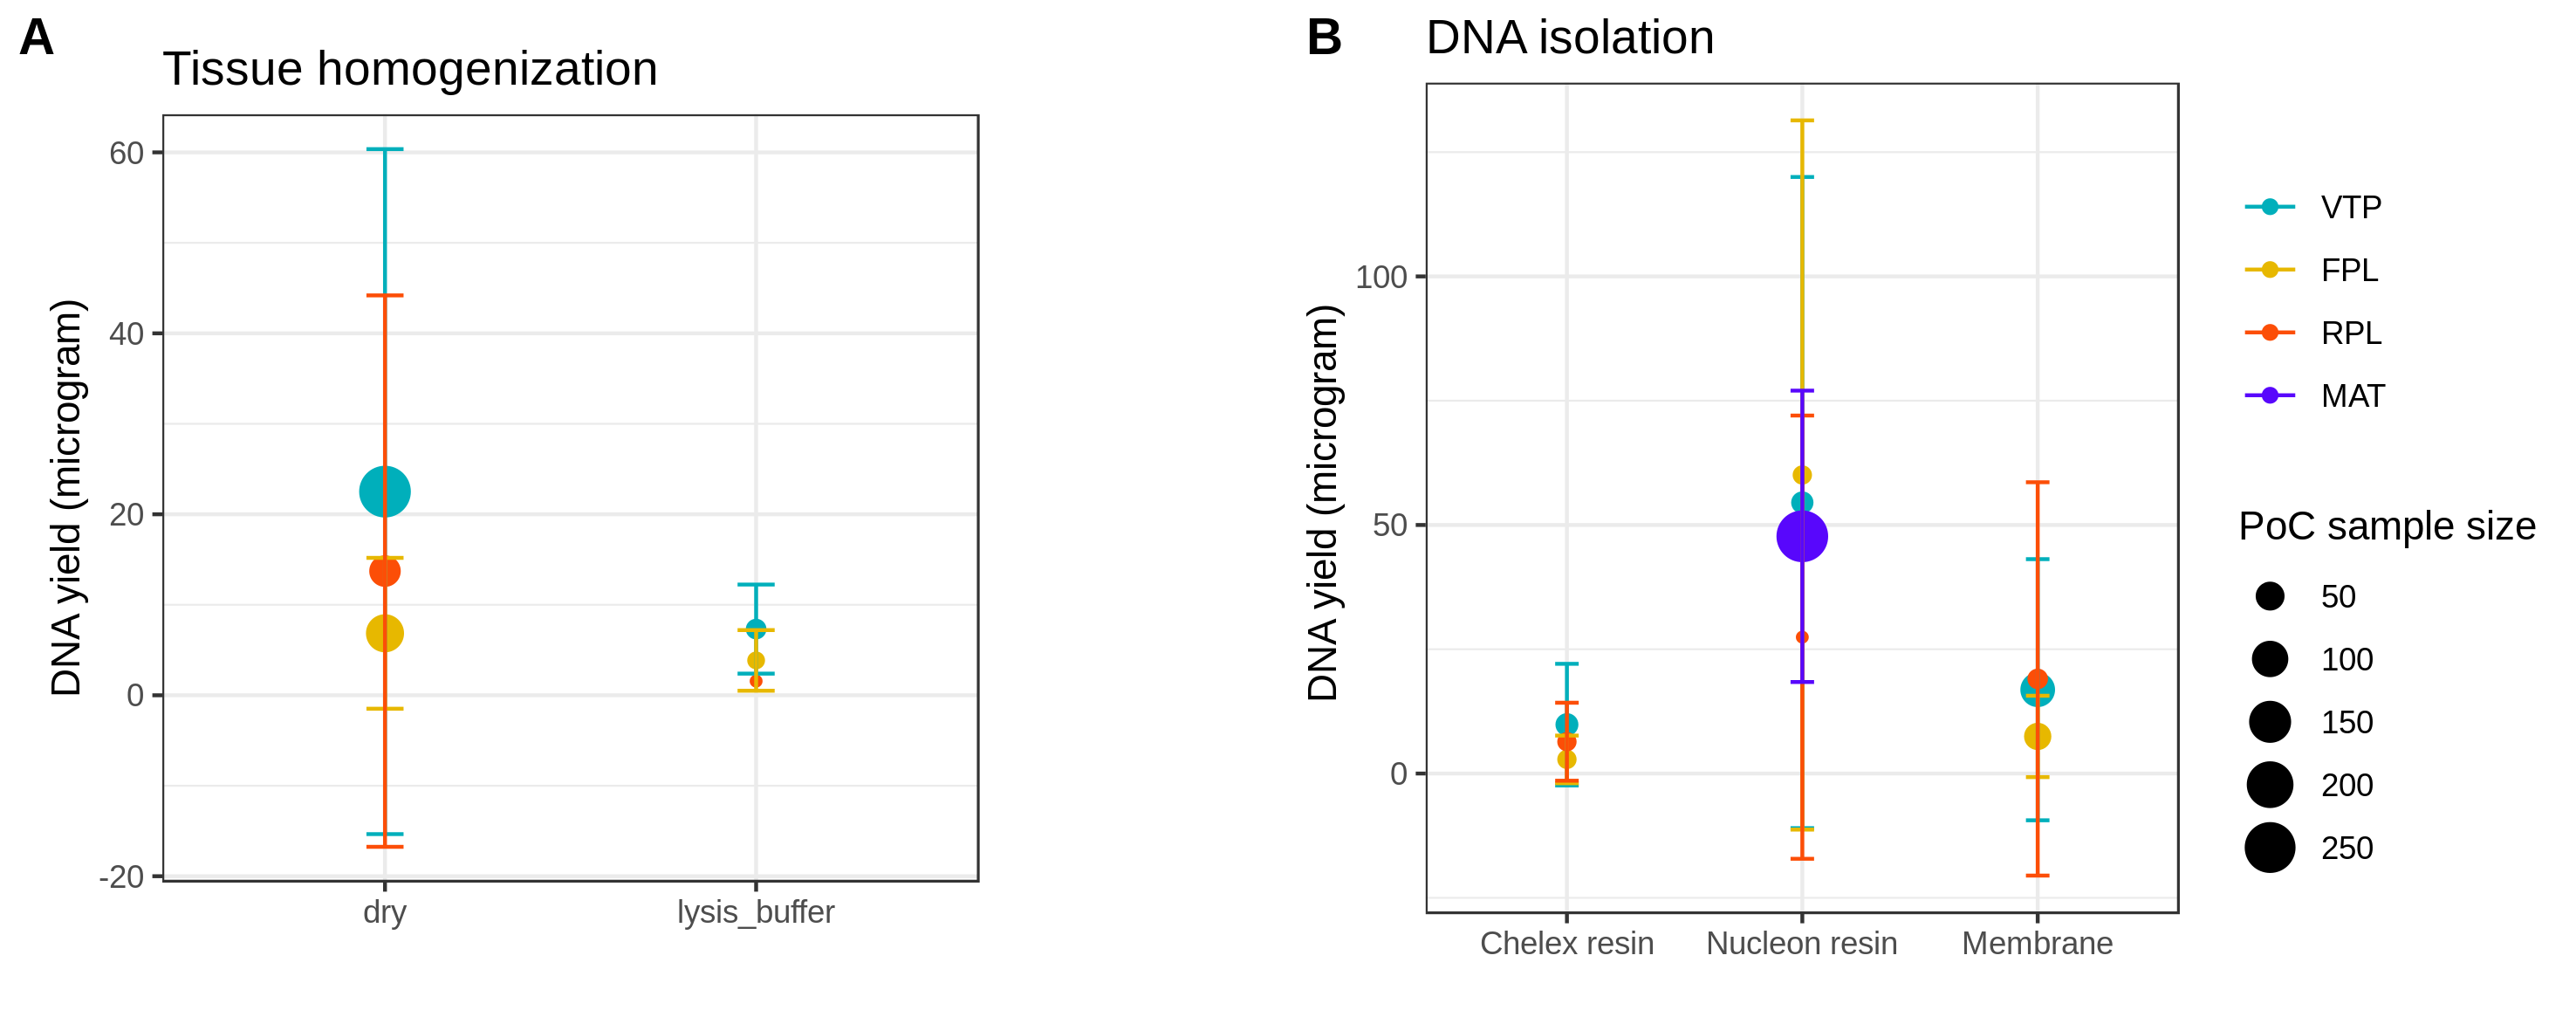
\includegraphics[width= 14 cm, high= 16cm]{fig/panelDNA.png}
    \caption{\textbf{Optimization of tissue homogenization and DNA extraction.} We do not observe significant difference between two methods of tissue homogenization (\textbf{A}), and three methods of DNA isolation (\textbf{b}) apart form a slightly higher range of yield for one type of resin. VTP: voluntary pregnancy termination;  FPL: first pregnancy loss; RPL:recurrent pregnancy loss;  MAT: maternal bllod; PoC: product of conception.}
    \label{fig:dna}
\end{figure}

\begin{figure}[ht]
    \centering
    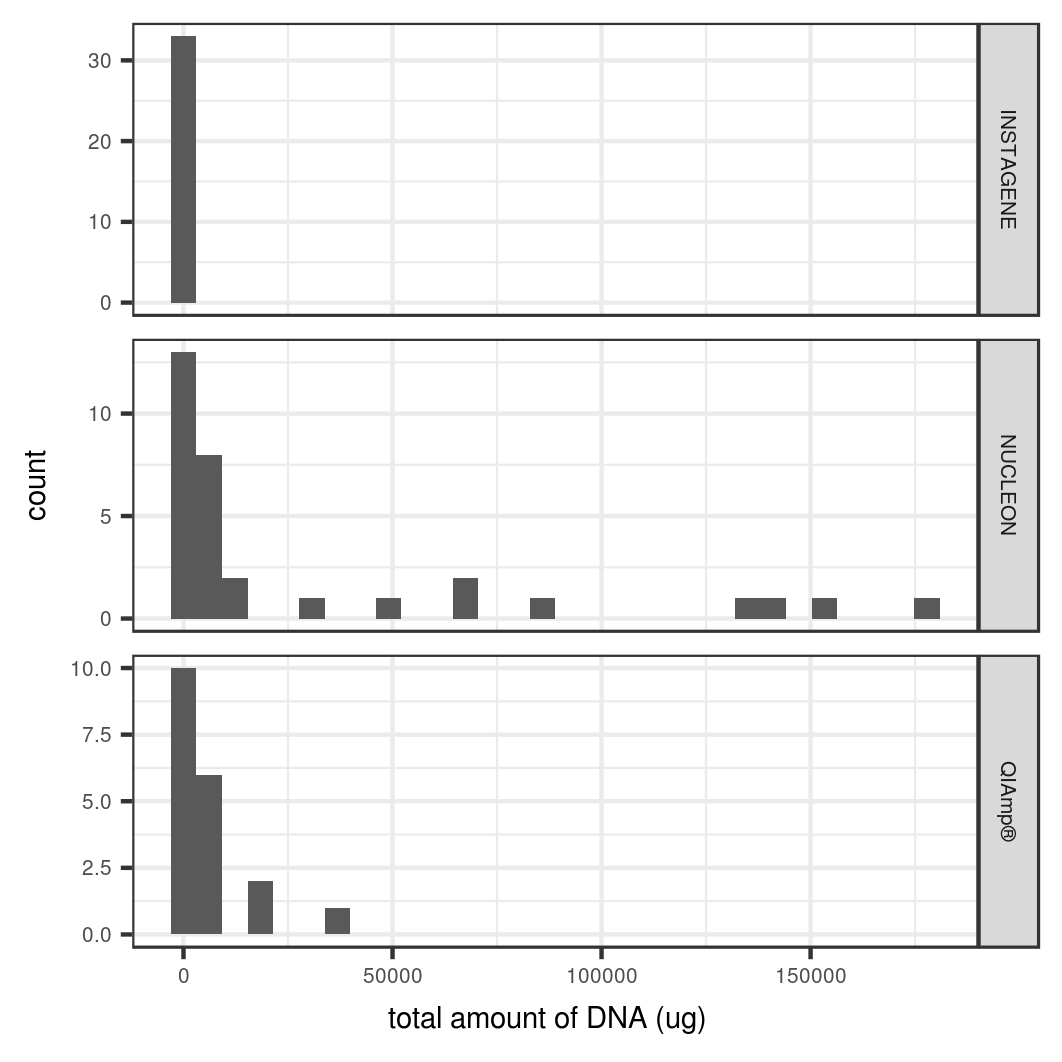
\includegraphics[width= 14 cm, high= 16cm]{fig/totaldna_bykit.png}
    \caption{\textbf{Yeld of DNA extraction form chorionic villi by extraction kit.} Distributions of total DNA as quantified using the  Qubit 2.0 Fluorometer} 
    \label{fig:dnayeld}
\end{figure}

\begin{figure}[ht]
    \centering
    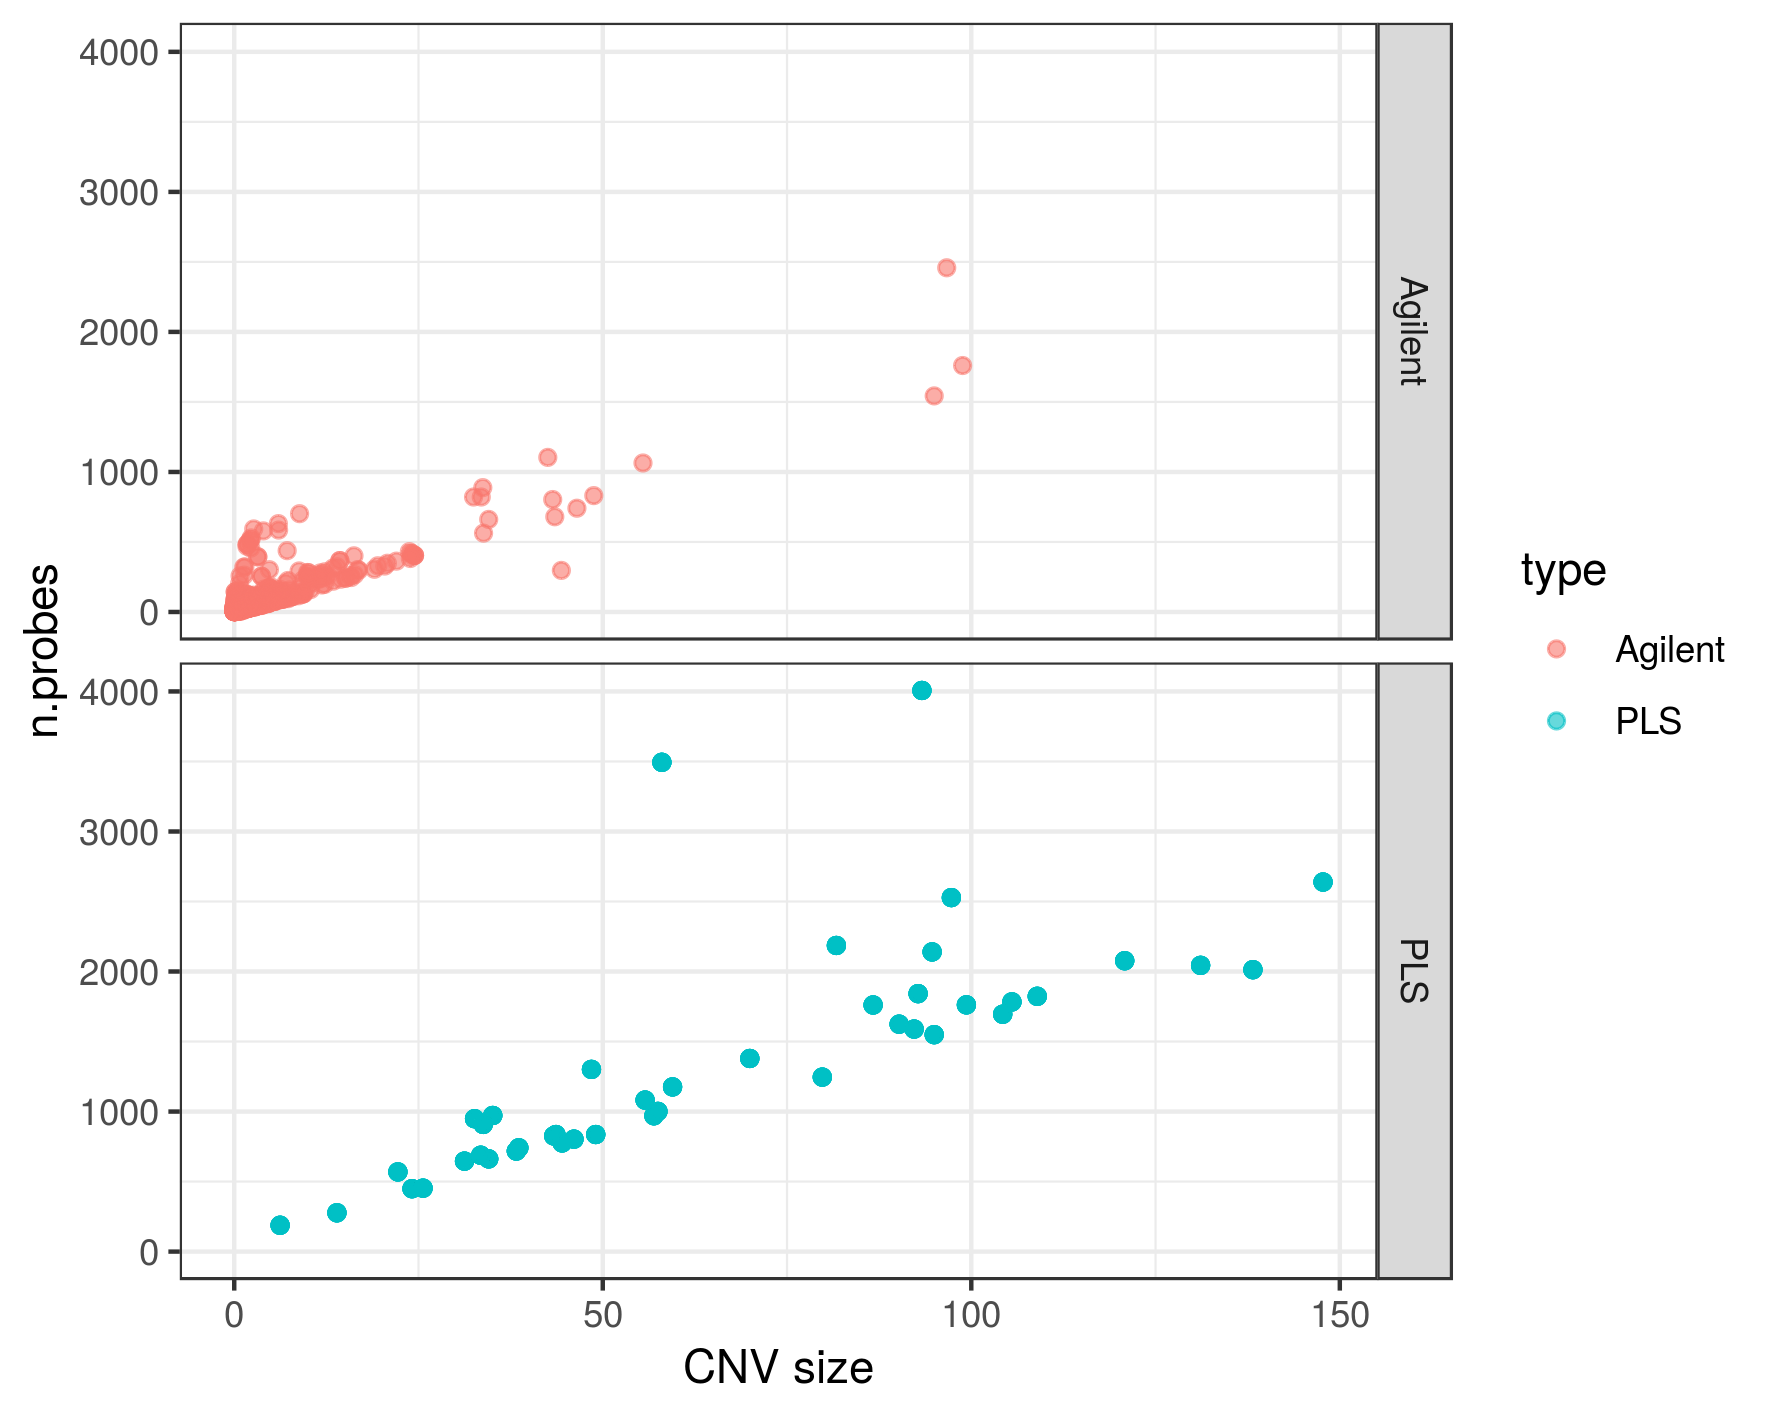
\includegraphics[width= 14 cm, high= 16cm]{fig/cnvCallComparison.png}
    \caption{\textbf{Copy number variant detection.} Comparison of calls made by the Agilent software and the penalized least square method implemented in the copynumber R package \cite{nilsen2012copynumber}} 
    \label{fig:cnvmethods}
\end{figure}


\end{document}